\documentclass{article}
\usepackage[utf8]{inputenc} %кодировка
\usepackage[T2A]{fontenc}
\usepackage[english,russian]{babel} %русификатор 
\usepackage{mathtools} %библиотека матеши
\usepackage[left=1cm,right=1cm,top=2cm,bottom=2cm,bindingoffset=0cm]{geometry} %изменение отступов на листе
\usepackage{amsmath}
\usepackage{graphicx} %библиотека для графики и картинок
\graphicspath{}
\DeclareGraphicsExtensions{.pdf,.png,.jpg}
\usepackage{subcaption}
\usepackage{pgfplots}
\title{AUTHORS\ \ $\Psi  $}
\author{@pcheltas, @lZzZzZzZzZzZl}
\date{June 2023}
\begin{document}
\maketitle
\newpage
% 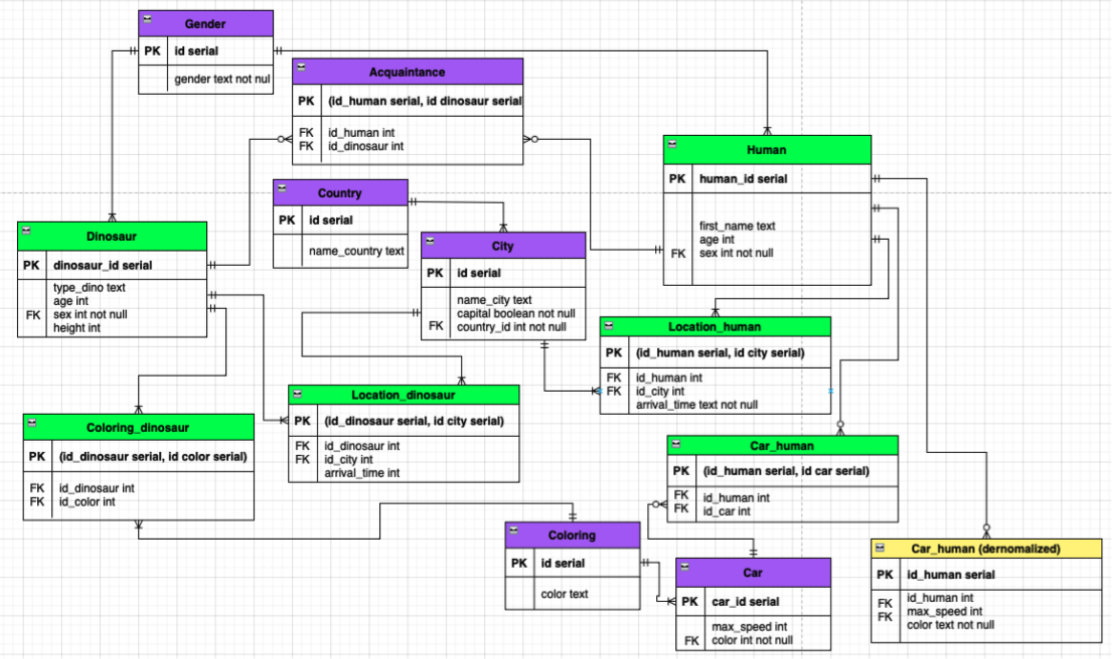
\includegraphics[width=.9\textwidth]{123}
\section{Две формы представления информации. Способы представления дискретной информации. Системы счисления, используемые в вычислительной технике: двоичная, 8-я, 10-я, 16-я, двоично-десятичная.}


Первая форма представления информации называется аналоговой или непрерывной. Количество значений, которые может принимать величина, бесконечно велико, даже если величина изменяется в ограниченном диапазоне. 
Слово непрерывность выделяет основное свойство таких величин – отсутствие промежутков между значениями. Величина представляется в виде одного сигнала, пропорционального этой величине. Используется в аналоговых вычислительных машинах.


Вторая форма представления информации называется цифровой или дискретной.
В отличие от непрерывной величины количество значений дискретной величины всегда будет конечным. Величина представляется в виде нескольких сигналов, каждый из которых соответствует одной из цифр.
Эта форма представления используется в ЭВМ.


Примером дискретной информации может служить, например, изображение, напечатанное с помощью принтера и состоящее из отдельных точек разного цвета. 
Примером дискретного хранения звуковой информации является аудиокомпакт-диск.


Системы счисления, используемые в вычислительной технике: двоичная, 8-я, 10-я, 16-я, двоично-десятичная являются примером представления дискретной инф.

Представление информации в привычной для нас десятичной сс значительно усложняет архитектуру, тк устройство в таком случае должно будет различать огромное количество состояний.
Двоичная: 0 или 1 для каждого бита, либо есть сигнал, либо его нет, является основной для ЭВМ\\
Восьмеричная: от 0 до 7. Широко использовалась в программировании, но позднее была почти полностью вытеснена шестнадцатеричной.\\
Десятичная: Не до конца удобная для машины, однако понятная для человека, при написании кодов, мнемоник\\
Шестнадцатеричная: от 0 до F. Удобна, поскольку минимальной адресуемой единицей памяти является байт (8 бит), значения которого удобно записывать двумя 16-ричными цифрами. \\
Двоично-десятичная: Используется для хранения десятичных чисел в памяти компьютера. Десятичная цифра задается 4 битами (от 0000 до 1001).
Удобно для вывода чисел на индикацию. Требует больше памяти. Усложнены арифметические операции.


\section{Представление чисел с фиксированной точкой. Прямой, обратный и дополнительный код. Формирование битовых признаков переноса, переполнения, отрицательного результата, нуля.}
В ЭВМ в основном используются три вида представления чисел – числа с фиксированной точкой, плавающей и строка символов. 
Особенностью представления чисел с фиксированной точкой является то, что они должны размещаться в разрядной сетке. 
В зависимости от положения точки определяется вес каждого символа в зависимости от заданной сс.
С помощью фиксированной точки представляются как целые, так и вещественные числа.


Прямой код числа – обычное его представление в заданной сс, обратный – инвертированный прямой код. 
С помощью дополнительного кода представляются отрицательные числа, что, в свою очередь упрощает конструкцию АЛУ. 
Именно обратный код обычно используется в вычислительных машинах. 
Доп код положительного числа равен самому числу, для отрицательных – дополнение до максимального положительного числа +1. 
Простейший способ вычислить доп код числа – инвертировать его и прибавить 1.


По окончании выполнения операции с числами устанавливаются признаки результата. 
Признаки отрицательного результата и нуля понятны исходя из их названия: отрицательность устанавливается по старшему биту результата (1-отрицательное, 0-положительное), 
ноль – при всех битах сетки равных 0. Существуют такие явления как перенос и переполнение. 
Перенос – для беззнаковых чисел, является признаком выхода за размерную сетку. 
Переполнение – для знаковых. Формируется как сложение по модулю 2 поразрядных переносов в старший и из старшего разрядов. 

\section{Представление символьных и строковых данных. Принципы построения кодовых таблиц ASCII, КОИ-8, ISO8859-5, Windows-1251, UTF-8, UTF-16.}
В ЭВМ представление текстовой информации основывается на кодировании букв и символов при помощи кодовой таблицы, где каждому символу соответствует номер. 
Шрифты бывают растровые – не могут масштабироваться и векторные – которые чертятся последовательностью линий в пределах заданной площади.


ASCII:\\
Порядковые номера 0-31 для них коды символов 00000000-00011111: являются управляющими символами для вывода.\\
Порядковые номера 32-127 для них коды символов 00100000-01111111: строчные и прописные буквы латинского алфавита, десятичные цифры, знаки препинания, скобки и другие символы.\\
Порядковые номера 128 — 255 для них коды символов 10000000-11111111: нелатинский алфавита


КОИ-8:\\
восьмибитовая кодовая страница, совместимая с ASCII 

Разработчики КОИ-8 поместили символы русского алфавита в верхней части таблицы таким образом, 
что позиции символов кириллицы соответствуют их фонетическим аналогам в английском алфавите из нижней части таблицы.


ISO – 8859-5:\\
8-битная кодовая страница

Нижняя часть таблицы кодировки соответствует кодировке ASCII (совпадает начало, потому что ASCII 7 ми битная). 
Основной недостаток - отсутствие некоторых символов, такие как тире, кавычки-ёлочки, градус.


Windows-1251:\\
Windows-1251 как и KOI8-R выгодно отличается от других 8‑битных кириллических кодировок CP866 и ISO 8859-5 наличием практически всех символов, использующихся в русской типографике.
Минусы - отсутствие символов псевдографики и совпадение буквы я со служебным символом в других кодировках.


Unicode – стандарт, определяющий таблицу символов в соответствие значение в виде U+число в 16сс. 
\\UTF-8:\\
кодировока текста, которая позволяет хранить символы Юникода, используя переменное количество байт. 
Совместимость с ASCII — любые их 7-битные символы отображаются как есть, а остальные выдают пользователю мусор.
\\Кодирование UTF-8:\\
1. Определить количество октетов, требуемых для кодирования символа. Номер символа берётся из стандарта Юникода.\\
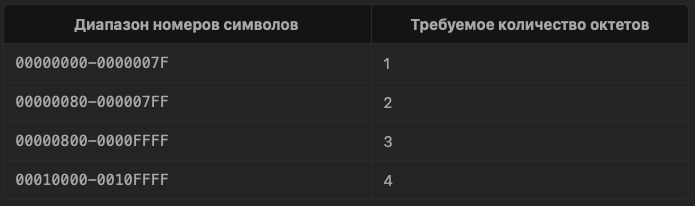
\includegraphics[width=.7\textwidth]{utf81.png}\\
2. Установить старшие биты первого октета в соответствии с необходимым 
количеством октетов:\\
Если для кодирования требуется больше одного октета, то в октетах 2-4 два 
старших бита всегда устанавливаются равными $10_2$ (10xxxxxx).\\
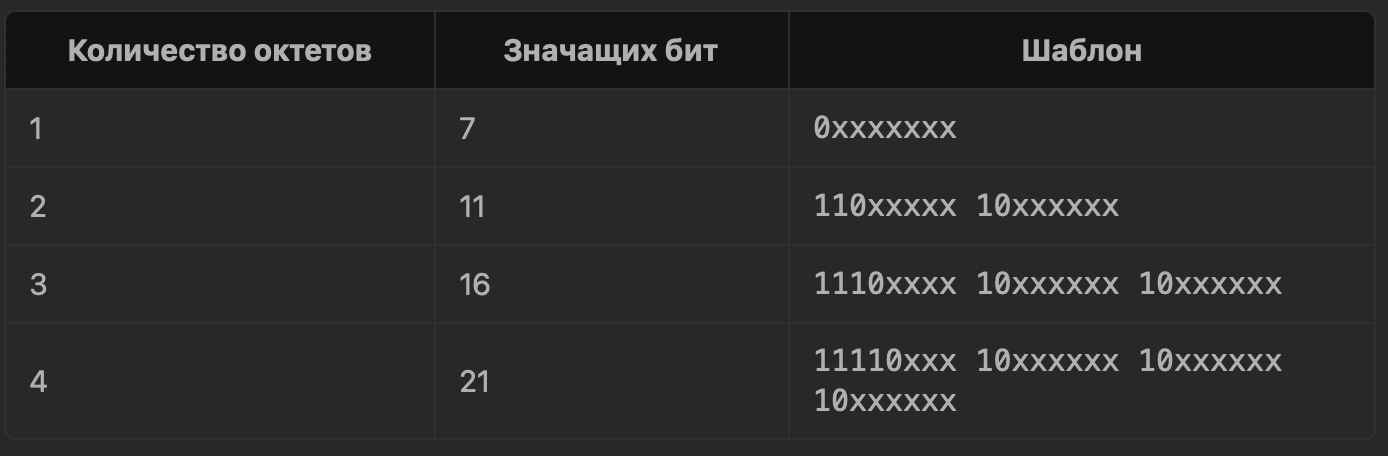
\includegraphics[width=.7\textwidth]{utf82.png}\\
3. Установить значащие биты октетов в соответствии с номером символа Юникода, 
выраженном в двоичном виде.


UTF-16:\\
символы кодируются двухбайтовыми словами с использованием диапазонов
значений $0$ от до $FFFF_{16}$.

Сдвигаем символ в 8 дипазонах $0000_{16}...D7FF_{16}$ и $E000_{16}...10FFFF_{16}$. 
Диапазон $D800_{16}...DFFF_{16}$ используется для символов, которые кодируются двумя 16 - битными словами.\\
Символы Unicode до $FFFF_{16}$ включительно записываются как есть 16-битным словом. Символы же в диапазоне $10000_{16}...10FFFF_{16}$ кодируются парой 16-битных
слов. Для этого их код арифметически сдвигается до нуля. В результате получится значение от нуля до FFFFF, которое занимает до 20 бит. Старшие 10 бит этого значения идут в лидирующее слово
, а младшие 10 бит — в последующее. При этом в обоих словах старшие 6 бит используются для обозначения суррогата. Биты с 11 по 15 имеют значения $11011_2$ , а 10-й бит содержит 0 у лидирующего слова и 1 - у последующего.

\section{Базовые элементы вычислительной техники: ячейки, регистры, шины, вентили, тактовые генераторы, логические схемы, триггеры, регистры, счетчики, сумматоры.}
Ячейка памяти – минимальный адресуемый элемент запоминающего устройства ЭВМ.
Они имеют адрес, по которому к ним могут обращаться команды процессора.


Регистр процессора – память внутри процессора, предназначенная для хранения адресов и промежуточных результатов вычислений или данных, необходимых для работы самого процессора. 
Операция чтения информации - создание копии его содержимого.


Шина - цепь, соединяющая регистр с другим регистром или иным устройством ЭВМ, может включать несколько проводов.
Также шина содержит несколько дополнительных проводов, используемых для передачи сигналов синхронизации и управления.


Вентильные схемы – ключевые схемы, предназначенные для управления потоком информации из регистров. Есть два входа для информационного сигнала и для управляющего, который разрешает/запрещает прохождение данных.


Тактовый генератор генерирует импульсы заданной частоты. Используется для синхронизации процессов передачи информации между устройствами.


Логическая схема - простейшее устройство ЭВМ, выполняющее одну определённую операцию над входными сигналами.


Триггер — класс электронных устройств, обладающих способностью длительно находиться в одном из двух устойчивых состояний и чередовать их под воздействием внешних сигналов. 


RS-триггер назвается по названию своих входов. Вход Set — позволяет устанавливать выход Q в единичное состояние. 
Вход Reset — позволяет сбрасывать выход Q — выход в нулевое состояние. Если он синхронный, то он будет пропускать входные сигналы только при наличии синхронизирующего сигнала.
\\
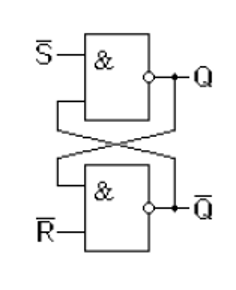
\includegraphics[width=.2\textwidth]{RS1}\\


D-триггер. При записи и хранении данных один бит может принимать значение, как нуля, так и единицы.\\


T-триггер — это счетный триггер. У данного триггера имеется только один вход. После поступления на
вход T импульса, состояние триггера меняется на прямо противоположное.


Счётчик числа импульсов — устройство, на выходах которого получается двоичный код. 
Счетчики импульсов являются разновидностью регистров и строятся на триггерах.


Сумматор — устройство, преобразующее информационные сигналы в сигнал, эквивалентный сумме этих сигналов.
Имеет 3 входа (2 операнда и бит переноса) и 2 выхода (результат сложения и бит переноса).



\section{Структура и принцип функционирования ЭВМ. Порядок функционирования простого процессора на примере калькулятора.}

Типичная ЭВМ состоит из процессора, памяти и устройств ввода-вывода. Сердцем ЭВМ является процессор, в состав которого входят устройство управления выборкой команд и их выполнением, алу, 
регистры, осуществляющие временное хранение данных и состояний процессора, схемы для управления и связи с системами памяти и ввода-вывода. 


Устройство ввода обеспечивает считывание информации. 
Устройства вывода представляют результаты обработки информации. 

Память ЭВМ включает устройство, обеспечивающее хранение команд и данных.
В микро ЭВМ используются безадресные, адресные команды, команды ввода-вывода и ветвления.


В процессе работы ЭВМ последовательно выполняет набор достаточно простых операций: 
выборку команды, выборка адреса, выборка операнда, выполнение, прерывание и ввод-вывод.
\\
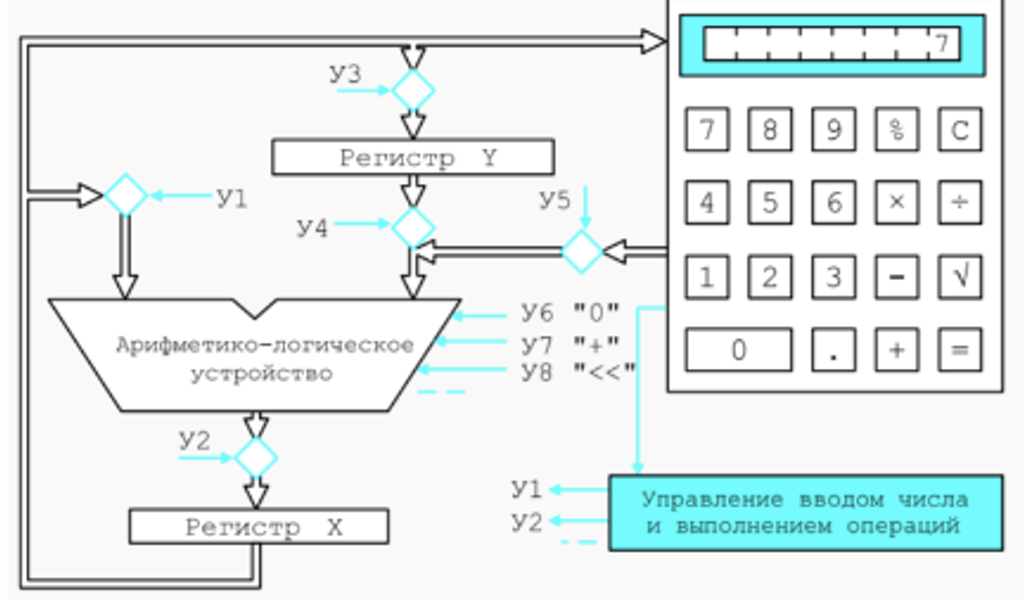
\includegraphics[width=.5\textwidth]{calc.png}\\

Калькулятор состоит из двух регистров X, Y, ALU, шин, вентелей. Любое нажатие запускает устройство управления, которое формирует последовательность импульсов для выполнения нужной операции. Допустим пользователь нажал цифру. 
Сначала пересылается содержимое X в Y (у3), далее обнуляется регистр X (у2, у6), который далее складывается с цифрой с клавиатуры (у1, у5, у7) и результат сохраняется в Х (у2).


Для ввода последующих цифр, нужно сдвинуть Х на 1 разряд (у1, у8). Запишем результат в X (у2) и сложим с цифрой с клавиатуры (у1, у5, у7) и сохраним результат в Х (у2)


При нажатии + или = нужно сложить содержимое регистров X и Y (y1, y4, y7) и сохраняется результат в Х.




\section{Операционная система Unix — ядро ОС и файловая система}
UNIX – семейство ос. Одна из основных ее заслуг – мультиплатформенность. Ядро можно адаптировать почти под любой микропроцессор.\\
Каждая операционная система выполняет служебные операции в ядре. Ядро представляет собой набор подсистем, которые управляют оборудованием и программами пользователя.


Основными подсистемами, которые жизненно важны для любой ОС являются управление памятью, управление процессами и потоками (отвечает за выполнение нескольких программ одновременно на одной ОС), 
виртуальная файловая система (обмен данными организован с помощью файлов, с точки зрения ОС B UNIX все является файлами), 
сетевая подсистема, драйвера устройств и платформо-зависимый код (драйвера, которые поддерживают функционирования системы на различных аппаратных архитектурах). 
Взаимодействие программ пользователя с ядром происходит с помощью интерфейса системных вызовов.


Файловая система UNIX представляет собой совокупность файлов, напоминающих дерево. 
Все в файловой системе является файлом, в том числе директории и каталоги. 
При этом каждый файл имеет свой собственный уникальный номер inode, а также путь. 
Путь может быть абсолютным – содержащим полный путь от корневой директории и относительным – начиная от текущего файла рабочего каталога. 
В каждом каталоге содержатся по умолчанию 2 файла: «.» - ссылка на самого себя и «..» - ссылка на родительский каталог. 
Ссылки в свою очередь бывают жесткими – они обладают тем же inode, что и исходный файл, существуют вне зависимости от его положения и содержат всю информацию о файле за исключением имени файла и его данных. 
Символически ссылки имеют свой собственный код и содержат только путь к заданному файлу.




\section{Операционная система Unix — основные команды, права файлов и способы их задания.}
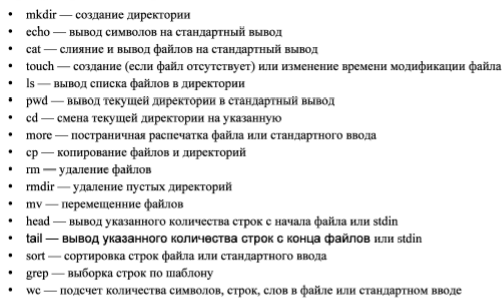
\includegraphics[width=.7\textwidth]{unixkom.png}\\
Права определяют доступ к файлам для разных типов участников. 
Права делятся на права владельца, группы и остальных, каждый из которых состоит из чтения, записи и исполнения. 
Исполнение для файла означает исполнение содержимого или переход в директорию. 
Права задаются с помощью команды chmod и по умолчанию все файлы имеют права rw-r—r--, если маска задания прав не была изменена. 
Их можно задавать числовым значением или прибавлением(отниманием)/присвоением данному участнику какого либо из прав.
\\
\\Для выставления прав файлу используется команда chmod. Существует 3 способа задания прав доступа:
\\chmod [ugoa]\{+-=\}[rwx] файл
\\Добавляет, удаляет или устанавливает выбранную комбинацию прав для выбранной комбинации категорий.
\\chmod число файл
\\Устанавливает права на основе восьмиричной записи.
\\chmod категория1=категория2 файл
\\Копирует права одной категории и присваивает их другой.




\section{Операционная система Unix — интерпретаторы, стандартные потоки ввода вывода, фильтры.}
Командный интерпретатор – программа, предоставляющая пользователю интерфейс для общения с командной строкой; 
эта программа переводит введенные команды на понятный операционной системе язык.


Интерпретатор более известен как оболочка. Наиболее распространенными оболочками являются sh, bash и shell.
Команды могут задаваться как напрямую в командной строке, так и поступать из стандартного ввода или указанного файла. 
Оболочка отвечает за перенаправление потоков ввода- вывода. В совокупности с набором утилит, она представляет собой операционную среду, 
язык программирования и средства решения как системных, так и прикладных задач.


Для взаимодействия и обмена информацией с пользователем используются файлы, именуемые стандартными потоками ввода и вывода.
Вывод на экран представляется тоже как запись в файл, а ввод – как чтение из файла. Кроме потоков ввода и вывода существует так же стандартный поток ошибок, на который выводится вся служебная информация. 
Стандартные потоки привязаны к файловым дескрипторам с номерами:
0 для stdin, 1 для stdout, 2 для stderr.


Потоки по умолчанию связаны с терминалом, но их можно подключить к чему угодно. 
В интерпретаторе такая операция называется перенаправлением.
Для осуществления перенаправления используются следующие операции:\\
\\
Команда > файл (или >>)\\
Выполняется команда, а вывод помещается в файл (или добавляется в конец).\\
\\
Команда < файл\\
Файл используется в качестве источника ввода. При этом на каждый запрос ввода программы считывается 1 строка текста из файла.\\
\\
Команда1 | команда2\\
Вывод команды1 пойдет в качестве ввода на команду2 без использования промежуточных файлов. Такая возможность называется конвейером.
\\ \\
Команда 2> файл\\
Поток ошибок направляется в файл. По умолчанию этот поток выводится на стандартный вывод.
\\ \\
Команда $2>\&1$ файл\\
Такой синтаксис используется для объединения потоков вывода и потока ошибок для обработки их вместе.
\\ \\
Вместе с ос Unix поставляются утилиты которые могут осуществлять фильтрацию данных. 
Командами-фильтрами являются grep – осуществляет выборку строк совпадающих с шаблоном регулярного выражения и sort – осуществляет сортировку строк по заданному условию. 

\section{Состав и структура БЭВМ. Адресные пространства БЭВМ. Система команд БЭВМ, форматы команд. Машинные циклы.}
БЭВМ – ЭВМ аккумуляторного типа, выполняющая простейшие операци с 16-разраядными словами.
Память – 2048 ячеек с адресами от 000 до 7FF. Процессор – состоит из ряда регистров, алу с коммутатором и блоком установки признаков результата а также устройства управления.
Устройство управления – выполняет команды процессора с помощью открытия вентелей и проверки битов заданного регистра в зависимости от типа микрокоманды (управляющая и операционная).


Арифметико-логическое устройство может выполнять арифметические операции, такие как сложение и сложение с учетом переноса, 
операции логического умножения и инвертирования, алу подключено к аккумулятору. Коммутатор выполняет операции передачи информации между байтами слова,
осуществления арифметических и циклических побитовых сдвигов, а также для расширения знака.


Блок установки признаков результата предназначен для формирования признаков результата NZVC, которые сохраняются в 4-х младших битах PS.


Аккумулятор - 16-ти разрядный регистр, являющийся одним из главных элементов бэвм. 
Результаты арифметико-логических операций обычно помещаются в АС.


Счетчик команд - регистр, который хранит адрес ячейки, содержащей следующую исполняемую команду программы.


Регистр адреса - 11-ти разрядный регистр, служит для организации обращений к ячейкам памяти.

Клавишный регистр - 16-разрядный регистр, предназначен для ввода адреса программы, 
кодов программы. Пульт содержит набор клавиш, позволяющих осуществлять ввод данных, 
запуск программы на выполнение и управление режимами работы БЭВМ.


Регистр состояния - 16-разрядный регистр, хранит биты управляющие работой БЭВМ и признаки 
результата.\\
Адресация в эвм делится на:


Безадресные команды: 15-12 биты равны 0, 11-0 представляют расширение КОП.


Команды ввода-вывода: 15-13 биты равны 0, 12 равен 1, 11 равен 0, 10-0 равен адресу.


Команды ветвления: 15-12 биты равны 1, 11-8 равны расширению КОП, 7-0 равны смещению.


Команды с прямой загрузкой операнда: 15-12 биты равны КОП, 11-8 равны 1, 7-0 равны числу.


Адресная команда: 15-12 биты равны КОП, для абс адресации в 11 бите стоит 0, для относ адресации 1. В абсолютной в 10-0 битах указываем адрес, а в относительной 10-8 будет режим, 7-0 смещение.\\


При исполнении команды выполняется определенное количество микрокоманд. Цикл команды обычно включает один или несколько машинных циклов. 
Возможные состояния: выборка команды, выборка адреса, выборка операнда, исполнение, прерывания.



\section{Организация вычислений в БЭВМ. Сдвиги, арифметические и логические операции. Цикл выборки команды.}
Целые двоичные числа без знака (с фиксированной запятой) можно использовать для представления нуля и целых чисел. 
В 16-разрядном слове они могут изменяться от 0 до 65535. Целые двоичные числа со знаком используются, когда необходимы положительные и отрицательные числа. 
Отрицательные числа представляются в дополнительном коде. Сложение чисел со знаком
и без знака выполняется с помощью команды ADD. По команде INC к содержимому
аккумулятора прибавляется единица, а по команде DEC – единица вычитается. Если при этом
возникает перенос из старшего разряда, то в регистр переноса запишется 1, иначе 0. 
Вычитание может выполняться путем сложения уменьшаемого и доп
кода вычитаемого. Для изменения знака числа необходимо его инвертировать,
а затем прибавить единицу. Команда AND выполняет над каждым разрядом аккумулятора и содержимым ячейки логическое умножение. 
Команда позволяет выделять или очищать определенные биты слова. Команды ROL и ROR замыкают аккумулятор и
регистр переноса в кольцо и сдвигают все биты кольца влево или вправо. ASR смещает на один бит влево всё число, заносит 0 в младший бит, а в старый старший бит в признак результата С. 
ASR : АС0 -> C, AC15->AC14. Сдвигом числа можно реализовать операции умножения или деления на 2.


Выборка команды: IP -> BR, IP -> AR, BR+1 -> IP, MEM(AR) -> DR, DR -> CR. После этого произойдёт определение типа команды и, если адресная, опеределение вида адресации.





\section{Организация массивов данных. Режимы адресации. Цикл выборки адреса и операнда БЭВМ.}
Есть два типа массивов, реализуемых в БЭВМ:


1) Массив, хранящий в себе количество обрабатываемых ячеек - выбирается индексная ячейка,
содержащая адрес первого элемента массива. Дальше либо записывается число обрабатываемых
ячеек в доп. коде в любую выбранную ячейку, либо первый элемент массива переводится в доп.
код, пересылается в какую-нибудь ячейку, а потом мы работаем с ней.


2) Массив, содержащий в себе некоторый заданный стоп-символ\\ \\


Режимы адресации:


1) С прямой абсолютной адресацией  - в 11 бите 0, а в битах с 0 по 10 записано абсолютное значение адреса операнда в памяти. DR->AR, MEM(AR)->DR.


2) С относительной адресацией - в 11 бите 1, а биты 8-10 режим адресации. В биты 0-7 записано смещение (может быть и положительным и отрицательным).


2.1) Прямая относительная. SXT\_CR(0-7)->BR, BR+IP -> DR, DR -> AR, MEM(AR) -> DR.


2.2) Косвенная относительная. SXT\_CR(0-7)->BR, BR+IP -> AR, MEM(AR) -> DR, DR -> AR, MEM(AR) -> DR


2.3) Косвенная автоинкрементная. SXT\_CR(0-7)->BR, BR+IP -> AR, MEM(AR) -> DR, DR+1 -> DR, DR -> MEM(AR), DR-1 -> DR, DR -> AR, MEM(AR)->DR


2.4) Косвенная автодекрементная. SXT\_CR(0-7)->BR, BR+IP -> AR, MEM(AR) -> DR, DR-1 -> DR, DR -> MEM(AR), DR->AR, MEM(AR)->DR


2.5) Со смещением относительно стека. SXT\_CR(0-7)->BR, BR+SP -> DR, DR -> AR; MEM(AR) -> DR


2.6) С непосредственной загрузкой операнда в аккумулятор. Для такого формата биты 8-11 установлены в единицы. SXT\_CR(0...7)->BR, BR->DR


\section{Управление вычислительным процессом в БЭВМ. Команды ветвлений, цикл исполнения команды LOOP}
Управление вычислительным процессом в БЭВМ организовано с помощью команд перехода (ветвления). 
Они имеют код F0XX-F9XX, CEXX – безусловный переход, где ХХ – смещение перехода относительно IP. 
Они работают, анализируя флаги операции. Для сравнения двух чисел перед командами перехода используется команда CMP, 
которая сравнивает число А из AC и B из аргумента CMP. Она вычитает из А В и выставляет флаги NZVC по результату, 
не изменяя содержимое аккумулятора. BNC - проверка флага N==0, BNS - проверка флага N==1, BZC - проверка флага Z==0, BZS - проверка флага Z==1, BVC - проверка флага V==0, BVS - проверка флага V==1, BCC - проверка флага C==0, BCS - проверка флага C==1, BLT - переход если меньше, BGE - переход если больше или равно. При верности этих высказываний будет переход.


С помощью команды LOOP организуется цикл. Она декрементирует значение ячейки, содержащейся в аргументе, сравнивает ее с 0, 
и, если ее значение <=0, перепрыгивает следующую команду.\\
Цикл исполнения LOOP:


1)(Не ноль)\~ 0 + DR -> DR


2)(Не ноль)\~ 0 + DR -> BR, DR -> MEM(AR)


3)IF BR(15) = 0 THEN GOTO INT


4)IP+1 ->IP


5)GOTO INT





\section{Подпрограммы в БЭВМ. Цикл исполнения команд перехода и возврата из подпрограммы. Стек, передача параметров. Позиционно-независимый код. Загрузчик и библиотеки.}
В процессе исполнения кода необходимо производить одинаковые действия, 
которые можно выделить в отдельный кусок кода, который впоследствии можно вызывать из основной программы. 
Такой кусок кода в asm называется подпрограммой. Выгодно использовать подпрограмму, 
когда количество команд подпрограммы вместе со служебными командами вызова и возврата будeт меньше, 
чем если бы код подпрограммы мы копировали. Осуществление вызова подпрограмм вызывается с помощью команды CALL, а возврата – RET. 


Цикл исполнения CALL:


DR -> BR; IP -> DR; BR -> IP; (NOT NULL)\~0 + SP -> SP,AR; DR -> MEM(AR); GOTO INT


Цикл исполнения RET:


SP -> AR; MEM(AR)->DR; DR -> IP; SP + 1 -> SP; GOTO INT


При вызове подпрограммы в структуру данных под названием стек записывается адрес возврата, по которому после исполнения подпрограммы мы вернемся в основную. 
Стек загружается значениями по принципу - первый зашёл, последний вышел.


Первым способом передачи данных в/из подпрограмму/ы через аккумулятор. 
Вторым способом передачи параметров является использование стека. Адрес возврата всегда должен лежать сверху, поэтому загрузка параметров должна производиться перед вызовом подпрограммы - PUSH. 
Перемещение содержимого ячеек в аккумулятор - POP. Исопльзование согласования о вызовах sdcall, stdcall, fastcall значительно упростит работу с подпрограммой.


Позиционно-независимый код – код, который не изменяет своей работы при перемещении ее в разных областях памяти. 
Относительная адресация должна использоваться внутри программы, все внешние обращения – абсолютные.


Существует специальная часть операционной системы под названием загрузчик и динамический линковщик программ. 
В программе, когда потребовалась какая-то функция, динамический линковщик грузит в память библиотеку с необходимой функцией, 
связывает программу и библиотечную функцию, устанавливая адреса переходов. 
Библиотеки делятся на разделяемые  и архивные.





\section{Организация ввода-вывода в вычислительных системах. Инициализация обмена, передачи информации и завершение обмена. Драйверы.}
К шине периферийных устройств любого процессора подключаются контроллеры, которые управляют внешними устройствами, которые к ним подключены. 
Нельзя напрямую подключить ВУ к процессору. Технически возможно, но из-за разницы скоростей при управлении программным путем, большая часть времени процессор будет ожидать готовности подключенного к нему ВУ и ресурсы будут тратиться нецелесообразно. 
Эта проблема решена контроллером (подобие локального процессора, который управляет обменом с ВУ, хранит данные, статусную информацию в своих регистрах).


Ввод-вывод разделяется на программно-управляемый и управляемый аппаратурой.


При программно-управляемом обмене инициализация обмена бывает синхронной (в заданное время), асинхронной (проверка состояния готовности) и по прерыванию (при инициализации обмена приостанавливается выполнение текущей программы, производится ввод-вывод и возвращается к выполнению программы, которая исполнялась до этого). Обмен данными (прием и передача) может также быть организован синхронно, когда наличие данных на шине подтверждается специальным сигналом синхронизации с постоянной частотой, и асинхронно, с использованием сигналов готовности и/или подтверждения приема-передачи данных. Завершение обмена – синхронное (в ответ на системный вызов приходит сигнал окончания обмена синхронно с ним) и асинхронное (после системного вызова через какое-то время приходит сигнал окончания обмена).  


Внутри ОС помимо контроллера нужен драйвер, который организует данные, которые поступают с ВУ, и преобразует в вид, понятный ОС.  Они организуют совместную работу с устройством, поскольку «знают» о принципах устройства и работы как ОС, так и контроллера ВУ.



\section{Организация ввода-вывода в БЭВМ. Устройства ввода-вывода, команды}
В БЭВМ реализована только программно-управляемая передача данных. 
Существует 10 ВУ: таймер, устройство вывода, устройство ввода, 2 устройства ввода-вывода, текстовый принтер, бегущая строка, 
7-ми сегментный индикатор, клавиатура, цифровая клавиатура.


Между ВУ и процессором включены простейшие КВУ, каждый из которых содержит: 


дешифратор адреса;


логику управления КВУ;


регистр данных;


регистр состояния.


регистр управления, где разряд 3 - для разрешения прерывания и разряды 0-2, которые содержат номер вектора прерывания. 
Если прерывания разрешены командой EI и установлено разрешение прерывания от контроллера, то контроллер будет генерировать сигнал IntRq 
и выставлять номер вектора прерывания на шину адреса.


шина данных (Data0..7), по которым происходит передача данных в процессор или из процессора;


шина адреса, (Addr0..7), по которой передается адрес внешнего устройства от процессора к КВУ и номер вектора запроса на прерывание (Int\#) от КВУ к процессору,
 подтверждаемый сигналом выдачи вектора (IntV);


сигнал запроса прерывания (IntRq), сигнал ввода (Input), сигнал вывода (Output), начальный сигнал предоставления прерывания (IntSC), входящий цепочный сигнал предоставления прерывания (IntSCi\#), исходящий цепочный сигнал предоставления прерывания (IntSCo\#), сигнал готовности (Rdy), сигнал синхронизации (Syn).



Со стороны процессора к системной шине БЭВМ подключены:


дешифратор приказа, который преобразует приказ в КОП команды ввода-вывода в набор управляющих сигналов на шине.


регистр разрешения прерывания; 


регистр прерывания от КВу, по которому выполняется цикл прерывания;


логика управления шины БЭВМ предназначена для подключения и отключения приемо-передатчиков сигналов КВУ и процессора для осуществления обмена CPU с одним из контроллеров в один момент времени.


Команды ввода-вывода. Код операции представлен значением 0x1 в разрядах 12-15. 
В разрядах 8-11 располагается приказ на ввод-вывод, его 3 младших разряда декодируются аппаратно на дешифраторе приказов, 
а биты 0-7 кодируют адрес регистра контроллера ввода вывода, с которым осуществляется обмен. 
Операция возврата из прерывания IRET осуществляет восстановление из стека значений регистра состояния и счетчика команд.

Команда DI запрещает прерывания. Команда EI разрешает прерывания. Команда IN \#req осуществляет чтение из регистра ВУ по адресу.
Команда OUT \#reg осуществляет запись в регистр ВУ. Команда INT \#reg вызывает программное прерывание с вектором num.






\section{Организация асинхронного обмена в БЭВМ. Пример программы. Временные издержки асинхронного обмена}
Алгоритм программы асинхронного обмена: сначала проверяется готовность ВУ к обмену и, если оно готово, 
дается команда на обмен (ввод или вывод). ВУ сообщает о готовности установкой в единицу флага в контроллере ВУ. 
При асинхронном обмене ЭВМ должна тратить время на ожидание момента готовности, а так как готовность проверяется командным путем, 
то в это время ЭВМ не может выполнять никакой другой полезной работы по преобразованию данных что и является издержками асинхронного обмена в бэвм.


Пример программы:


START: CLA 

S1: IN 5

AND \#0x40

BEQ S1

IN 4

SWAB

ST RES 

S2: IN 5

AND \#0x40

BEQ S2

LD RES 

IN 4

ST RES

HLT

RES: WORD ?


\section{Организация прерываний в БЭВМ. Вектора прерываний, контроллер прерывания.}


В процессе исполнения основной программы готовность ВУ вызывает программно-аппаратный процесс, который после цикла исполнения команды переходит 
на цикл прерывания, останавливает текущую программу и переходит на специальную подпрограмму, которая запрещает прерывания, сохраняет текущее состояние АС и IP. 
После обмена по этому сохраненному состоянию будет произведено восстановление состояния, разрешение прерываний и продолжение исполнения программы 
с момента на котором мы остановились.


Если смотреть это детальнее: ВУ выставляет на свою шину сигнал требования прерывания, который сохраняется на процессоре в регистре состояния, пока не начнется цикл обработки прерывания. 
В цикле обработки прерываний проверяются некоторые входные параметры и как раз есть ли сигнал IntRq (бит в PS), после чего БЭВМ формирует управляющий сигнал предоставления прерываний (IntSC). 
Он проходит цепочкой насквозь всех ВУ, между входом и выходом проверяет был ли запрос прерывания у каждого ВУ (если был, то маскирует сигнал, не пропуская дальше и выставляет на шину адреса номер вектора своего прерывания). 
Будет происходить до тех пор, пока не будут обработаны все прерывания, которые установлены в контроллерах ВУ. 


Вектор прерывания – совокупность адреса программы обработки прерывания и его регистра состояния. 
В БЭВМ 8 типов прерываний, то есть 8 векторов, которые лежат от 000 до 00F включительно. Чтобы правильно инициализировать вектора прерываний, адреса в ячейках обработки прерываний всех векторов необходимо установить на подпрограмму. 
На одном векторе может быть несколько прерываний.


Контроллер прерываний контролирует вложенность прерываний и возможность их исполнения, то есть проверяет является ли новое прерывание более приоритетным, 
чем то, которое обрабатывается сейчас и вложенность, так как она ограничена. 


\section{Организация обмена по прерыванию программы в БЭВМ. Пример программы. Цикл прерывания.}



Обмен по прерыванию используется когда момент передачи данных заранее неизвестен. Обмен данными между ЭВМ и ВУ инициируется сигналом с ВУ.
 Для реализации данного типа обмена используется аппаратная проверка наличия внешнего прерывания, т. е. сигнала готовности по линии "Запрос прерывания". 
 По завершении цикла исполнения текущей команды происходит переход к циклу прерывания, который есть у всех команд кроме EI, DI и HLT. 
 Если в этот момент на линии «Запрос прерывания» нет сигнала о готовности ВУ или прерывания запрещены, то выполняется следующая команда. Иначе, прерывания запрещаются, 
 в ячейку с адресом 000 заносится содержимое СК, и управление передается команде, расположенной в ячейке 001, с которой начинается программа обработки прерываний. 
 Программа обработки прерываний запоминает в памяти содержимое A в ячейку SAVED\_A и содержимое С в ячейку SAVED\_C. 
 Т.е. минимальная информация о прерванной программе хранится в ячейках 000, SAVED\_A и SAVED\_C. 
 Логика состоит в поочерёдной провекри ВУ, если ВУ готово, то происходит обработка ВУ Нного, выполняется передача данных, сброс флага готовности ВУ и переход к проверке готовности следующего ВУ N+1.
В самом конце восстанавливается флаг прерываний для основной программы, который был до проверки прерываний.

\begin{minipage}{.5\textwidth}
    Цикл прерываний: 

    if PS (W) = 0 then GOTO STOP;
    
    if PS (INT) = 0 then GOTO INFETCH;
    
    INTS;
    
    (не ноль)\~0 + SP -> SP, AR
    
    IP -> DR
    
    DR -> MEM (AR)
    
    (не ноль)\~0 + SP - SP, AR
    
    PS -> DR
    
    DR -> MEM (AR);
    
    LTOL (CR) -> BR ;
    
    SHL (BR) -> BR, AR ;
    
    MEM (AR) -> DR;
    
    DR -> IP;
    
    LTOL (BR + 1) -> AR ;
    
    MEM (AR) -> DR;
    
    DR -> PS ;
\end{minipage}
\hfill
\begin{minipage}{.5\textwidth}
    Пример программы:

    VO: WORD \$DEFAULT, 0x180 
    
    V1: WORD \$INT1, 0x180
    
    V2: WORD \$DEFAULT, 0x180 
    
    V3: WORD \$INT3, 0x180
    
    \dots
    
    V7: WORD \$DEFAULT, 0x180
    
    DEFAULT: IRET
    
    START: DI
    
    CLA
    
    OUT 1
    
    OUT 5
    
    LD \#9
    
    OUT 3
    
    LD \#0xB
    
    OUT 7
    
    \dots
    
    JUMP \$PROG
    \\ 
    
    
    PROG: EI
    
    CLA
    
    INCLP: INC
    
    BR INCLP
    
    ORG 0x03F
    
    IO3: WORD?
    
    
    INT1: NOP
    
    PUSH
    
    ASI
    
    OUT 2
    
    POP
    
    NOP
    
    IRET
    
    INT3: NOP
    
    PUSH
    
    CLA
    
    IN 6
    
    ST \$I03
    
    NOP
    
    POP
    
    IRET
\end{minipage}

\section{Понятие многоуровневой ЭВМ. Понятие и пример программы на разных уровнях.}

Многоуровневая ЭВМ – это вычислительная машина, имеющая средства для работы с n различными уровнями языков программирования. 
Нижний язык, или уровень, является наиболее простым, верхний – наиболее сложным. 
Такую машину можно рассматривать как n различных виртуальных машин, каждая из которых имеет свой машинный язык. 
Сложность аппаратурной реализации этих виртуальных машин возрастает по мере увеличения номера уровня.
Рассмотрим различные уровни языков в бэвм, начиная с самого низкого. 

1. Микропрограммный уровень

2. Машинные команды

3. Язык ассемблера

4. Уровень проблемно-ориентировочных задач (алгоритмический язык)

5. Уровень программных систем (специальный язык)
\\
Рассмотрим примеры по обратной умерации.

5. X=Y+Z эксель

4. int ans = x + y; Java

3.

ORG  ...

X: WORD...

Y: WORD...

Z: WORD...

   LD Y

   ADD Z

   ST X

   HLT

4.

228 … (переменная X)

229 … (переменная Y)

230 … (переменная Z)

231 A229 

232 4230 

233 E228 

234 0100 

5.

32 0010E09011   ADD  AC + DR ? AC, N, Z, V, C
\section{Микропрограммный уровень БЭВМ. Структура МПУ. Форматы микрокоманд.}

На нижнем уровне БЭВМ выполняются микропрограммы. 
В каждом такте работы ЭВМ из памяти в регистр микрокоманд пересылается очередная 
микрокоманда, на которую указывает счетчик микрокоманд.

Структура МПУ: Есть память микрокоманд, в счетчике +1 , по его содержимому в памяти микрокоманд выбирается значение и поступает в регистр микрокоманд, 
в регистре выбирается тип команды и открывается определенный вентиль: 

1) операционная - все биты микрокоманды поступают на вентильные схемы 

2) управляющая -  часть в вентильные, значение регистра в устройство управления. 
Если проверяемый бит и бит из поля сравнения идентичны, то схема сравнения формирует единичный сигнал, который открывает вентильную схему ВА и на СчМК пересылается адрес перехода (16-24-ый биты УМК).
В противном случае на СчМК передается нулевое значение, которое инициирует увеличение значения СчМК на единицу (используется схема ИЛИ-НЕ для всех битов адреса перехода).


Биты 0-15 обоих типов совпадают, логика остальных разная. В 39-ый бит РМК записывается код операции, 0 - для ОМК; 1 - для УМК. Этот сигнал подается напрямую на вентили УМК (16-32 биты РМК) и через инвертор на вентили ОМК (16-35 биты РМК), открывая/закрывая биты УМК/ОМК, тем самым производя выбор типа микрокоманды.
Разряды РМК, содержащие 1, создают открывающий управляющий сигнал, а содержащие 0 - закрывающий. У битов 0-15 обоих типов микрокоманд назначение одинаковое, биты 0-7 отвечают за сигналы чтения регистров, регистры 8-11 отвечают за действия в АЛУ, биты 12-15 отвечают за сигналы передачи в коммутаторе. Далее назначение битов в каждом типе отличается:

ОМК: биты 16-23 отвечают за сигналы преобразований и установки флагов в
коммутаторе; биты 24-31 - запись в регистр результат преобразований; биты 32-33 - взаимодействие с памятью БЭВМ; биты 34-35 - взаимодействие с внешними устройствами; бит 38 - бит останова.


УМК: биты 16-23 - выбор бита для сравнения, работающий по схеме „ИЛИ" с данными поступающими из коммутатора; биты 24-31 задают адрес перехода, куда перейдет программа в случае, если схема инверсного „XOR" даст положительный результат (бит сравнения и результат схемы „И" выбора бита одинаковы); бит 32 - поле для сравнения с схеме инверсного „XOR".
\section{Структура и принципы работы арифметико-логического устройства и коммутатора. Регистр состояния БЭВМ}

У АЛУ есть два входа: левый и правый. К правому подключены регистры SP, IP, CR, DR, к левому -– AC, BR, SP, клавишный регистры. 
На каждом входе находятся инверторы, внутри есть схема сумматора и схема логического И, реализована операция инкремента и обратного кода. 


Из АЛУ на коммутатор поступают 18 разрядов результата (16 бит результата и биты, необходимые для формирования признака переноса С), а также предыдущее значение переноса из регистра состояния. Коммутатор, в свою очередь, выполняет сдвиги, операции расширение знака, а также операции прямой и перекрестной передачи информации между байтами.
 Информация из коммутатора поступает на шину данных записи в регистры БЭВМ и на блок установки признаков результата. 


Регистр состояния (PS - Program State) - 16-разрядный регистр, хранит биты управляющие работой БЭВМ (работа, прерывание и пр.) и признаки результата. В 5
актуальной программной реализации используются только 9 младших разрядов. Рассмотрим все 9 битов:

0 - бит переноса; 1 - бит переполнения; 2 - бит zero флага; 4 - используется для организации безусловных переходов в мпу; 5 - резрешение прерываний; 6 - прерывание (логическое и шины запроса на прерывание и бита 5 PS); 7 - состояние тумблера работа/останов; 8 - программа.



\section{Микропрограммное управление вентильными схемами. Схема управления. Интерпретатор БЭВМ.}

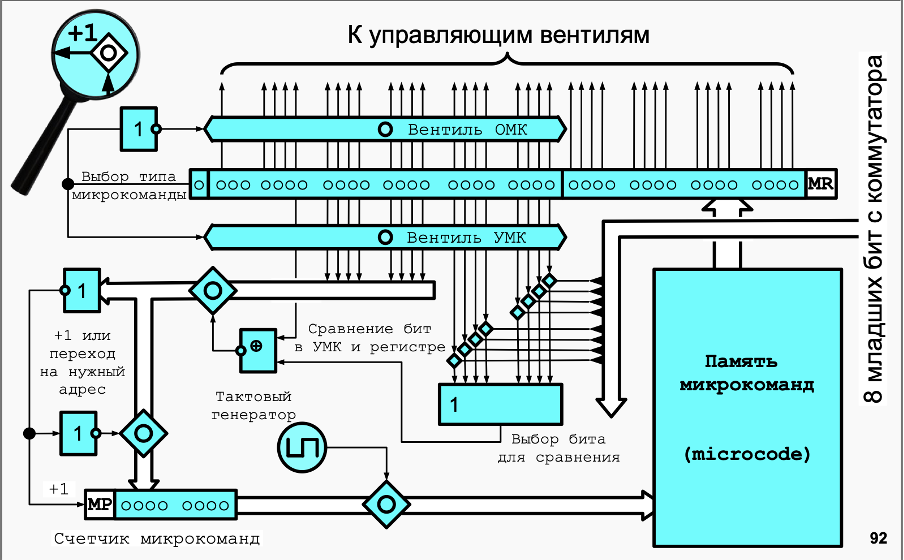
\includegraphics[width=1\textwidth]{mpu.png}\\
Содержимое памяти микрокоманд в каждом такте (тактовый генератор в середине) передается в регистр микрокоманд (MR, 40 разрядный). Младшие 16 разрядов (одинаковая часть независимо от типа микрокоманды) сразу передаются на управляющие вентили.
39й бит это код операции микрокоманды. Если он 0, то микрокоманда операционная. Этот бит подаётся вниз на вентиль УМК и вверх через инвертор на вентиль ОМК. Предположим, что наш 39 бит - 0. Тогда он поступает на инвертор, на выходе инвертора получается единица. Открывается вентиль ОМК. Оставшиеся биты тоже сваливают на управляющие вентили.
Предположим теперь, что код операции МК не 0, а 1. Откроется вентиль УМК. Среди тех бит, которые еще не ушли на вентильные схемы, рассмотрим младшие 8 (поле выбора проверяемого бита). 
Справа по шине передаётся 8 младших бит с коммутатора, которые поступают на вентили, которые открываются теми самыми 8 битами, которые отвечают за выбор проверяемого бита. 
Если происходит совпадение одного из 8 битов МК и одного из 8 битов коммутатора, соответствующий вентиль открывается. 
Прямоугольник чуть ниже вентилей - это одна большая схема ИЛИ. Результат идет на один из входов обратного ксора, который расположен немного выше тактового генератора. 
На второй вход этого же самого обратного ксора идет бит номер 32. Посмотрев на регистр MR понимаем, что это “однобитовое поле сравнения”.
Обратный ксор дает единичку, если два его входа совпадают. Таким образом, если два входа совпали, то открывается вентиль шины, на которую поступили 8 последующих битов из регистра MR.


Допустим вентиль открылся. Тогда адрес перехода проходит вентиль и идёт вправо на инвертор и вниз до вентиля, 
который ведёт к счётчику микрокоманд. Рассмотрим первый путь, если на инвертор подать 1, то далее нолик пойдёт вниз и прибавится к счётчику микрокоманд, 
по пути будет ответвление вправо, там стоит еще один инвертор, пройдя через который 0 станет 1 и, попадая на тот самый вентель, откроет его, 
поэтому адрес перехода пройдёт напрямую в счётчик команд.

Интерпритатор состоит из следующего:

1. Цикл выборки команд

2. Цикл выборки адреса операнда и обработки режимов адресации

3. Цикл выборки операнда

4. Цикл исполнения, куда входят:

- Декодирование и исполнение адресных команд

- Декодирование и исполнение ветвлений

- Декодирование и исполнение безадресных команд

5. Декодирование и исполнение команд ввода-вывода

6. Цикл прерывания

7. Пультовые операции

8. Свободные ячейки для:

- Арифметической команды

- Команды перехода

- Безадресной команды




\section{Архитектура ЭВМ. Гарвардская и фон-Неймановская архитектура. Организация обмена архитектуры ЭВМ с использованием шин.}

В разработке вычислительных систем есть два подхода к их построению: архитектура фон Неймана и Гарвардская архитектура.
Основным отличием между архитектурами является способ работы с памятью. В настоящее время в чистом виде архитектуры встречаются редко, 
обычно используется их комбинация в разных функциональных блоках ЭВМ.
В Гарвардской архитектуре центральным устройством является Control Unit - управляющее устройство в ЭВМ. 
Все остальные устройства ЭВМ подключены к управляющему устройству и взаимодействуют через него. 
Память для команд (instruction memory), данных (data memory) и устройств ввода вывода физически отделена друг от друга. 
В чистом виде такая архитектура уже не используется.
Используя такой подход нельзя нарушить логику программы, никогда не возникает путаницы между инструкциями и данными.


Архитектура фон Неймана содержит все в общей памяти. Нельзя определить, что находится в ячейке, данные или инструкции, без дополнительного анализа кода самой программы. 
При этом устройство обращения к памяти едино для данных и инструкций. 
Отдельно выделены устройства ввода вывода, которые являются внешними по отношению к процессору - объединению памяти, АЛУ и управляющего устройства.

Канальная организация обмена: Архитектура строилась вокруг памяти, она была центральным звеном. 
Скорость всех блоков вычислительной машины была примерно одинакова. С внешними устройствами работали отдельные процессоры. 
Блоки связаны шинами, работают независимо друг от друга. 


Раздельные шины: Через какое-то время производительность процессора стала больше чем памяти, поэтому процессор занял центральную позицию.
Он управлял памятью под тремя различными шинами. Скорость процессора и памяти повысилась, а контроллер внешних устройств остался примерно таким же. 


Общие шины: Отличием между 1,2 и третьим поколением является задача увеличения количества элементов и производительности на единицу объема. 
Для упрощения конструкции на одной шине стали располагаться все устройства кроме процессора. 


Мультиплексирование шин: Для сокращения количества проводов, которые соединяли блоки вычислительной машины, адрес и данные стали передавать по одним и тем же физическим проводам. 
В один импульс тактового генератора передавался адрес, в другой – данные. 


\section{Архитектура многопроцессорных ЭВМ. Системный коммутатор. Архитектуры UMA и NUMA}

UMA – архитектура современных машин. Технически UMА-системы предполагают наличие узла, 
соединяющего каждый из n процессоров с каждым из m модулей памяти. Простейший путь построения таких ВС - объединение нескольких процессоров с единой памятью посредством общей шины. 
В каждый момент времени обмен по шине может вести только один из процессоров. При использовании системной шины с несколькими процессорами возникла нехватка пропускной способности. 
Само использование нескольких процессоров обеспечивает возможность параллельной организации многих потоков команд и данных.

Коммутатор представляет собой несколько системных шин, каждая из которых подключена к отдельному процессору и остальным устройствам. 
Он в состоянии параллельно обслуживать несколько запросов. Каждый процессор может быть соединен со своим модулем памяти и иметь доступ к нему на максимальной скорости. 
Соперничество между процессорами может возникнуть при попытке одновременного доступа к одному и тому же банку памяти. 
В этом случае доступ получает только один процессор, а прочие - блокируются.


NUMA – предназначена для повышения количества процессоров. Каждый процессор организован с локальной памятью, локальным кэшем, своим тактовым генератором в виде единой сборки, платы. 
Все платы связаны друг с другом через коммутатор. Все процессоры работают под одной операционной системой, и вся память является общей, те при необходимости процессор может использовать память других системных плат, 
но скорость доступа к другим участкам памяти в отличие от локальной будет меньше. ОС заботится о том, чтобы данные сохраняли принцип локальности. 
Плюсами такой архитектуры является возможность работы процессоров на разной тактовой частоте, а также возможность на горячую менять компоненты вычислительной системы. 

\section{Структура современных процессоров. Окружение процессора. CISC, RISC, VLIW.}
Ядро процессора – основная часть, содержащая все функциональные блоки и осуществляющая выполнение всех логических и арифметических операций.
Принцип работы ядра процессора основан на цикле. В упрощенном виде этапы цикла работы ядра процессора можно представить следующим образом:

1. Блок выборки инструкций проверяет наличие прерываний. Если прерывание есть, то данные регистров и счетчика команд заносятся в стек, а в счетчик команд заносится адрес команды обработчика прерываний. 
По окончанию работы функции обработки прерываний, данные из стека будут восстановлены;

2. Блок выборки инструкций из счетчика команд считывает адрес команды, предназначенной для выполнения. По этому адресу из КЭШ-памяти или ОЗУ считывается команда. 
Полученные данные передаются в блок декодирования;

3. Блок декодирования команд расшифровывает команду. 
Если это команда перехода, то в счетчик команд записывается адрес перехода и управление передается в блок выборки инструкций (пункт 1), 
иначе счетчик команд увеличивается на размер команды и передает управление в блок выборки данных;

4. Блок выборки данных считывает из КЭШ-памяти или ОЗУ данные и передает управление планировщику;

5. Управляющий блок определяет, какому блоку выполнения инструкций обработать текущую задачу и передаёт её;

6. Блоки выполнения инструкций выполняют требуемые командой действия и передают управление блоку сохранения результатов;

7. При необходимости сохранения результатов в ОЗУ, существует блок сохранения результатов, который передаёт управление блоку выборки.

Описанный выше цикл называется процессом (именно поэтому процессор называется процессором). 


CISC - Концепция проектирования процессоров, которая характеризуется огромным количеством программ, одни отмирали и были не нужны, другие хранились с целью совместимости, в общей массе было невероятное количество хранимых команд. 
Процессору с архитектурой CISC приходится иметь дело с более сложными инструкциями неодинаковой длины. 
Выполнение одиночной CISC-инструкции может происходить быстрее, однако обрабатывать несколько таких инструкций параллельно сложнее.


RISC - процессор с сокращенным набором команд.
Все команды одинакового формата с простой кодировкой. Обращение к памяти происходит посредством команд загрузки и записи. 
Команда, поступающая в CPU, не требует дополнительной дешифрации. Большая часть программного обеспечения написана и откомпилирована специально для CISC-процессоров фирмы Intel.

VLIW - архитектура процессоров с несколькими вычислительными устройствами. 
Характеризуется тем, что одна инструкция процессора содержит несколько операций, которые должны выполняться параллельно, 
базируется на RISC-архитектуре. Несколько инструкций, упакованы в одну команду. 


\section{Адресуемая память, организация и временные диаграммы. Конструктивные особенности современной памяти.}
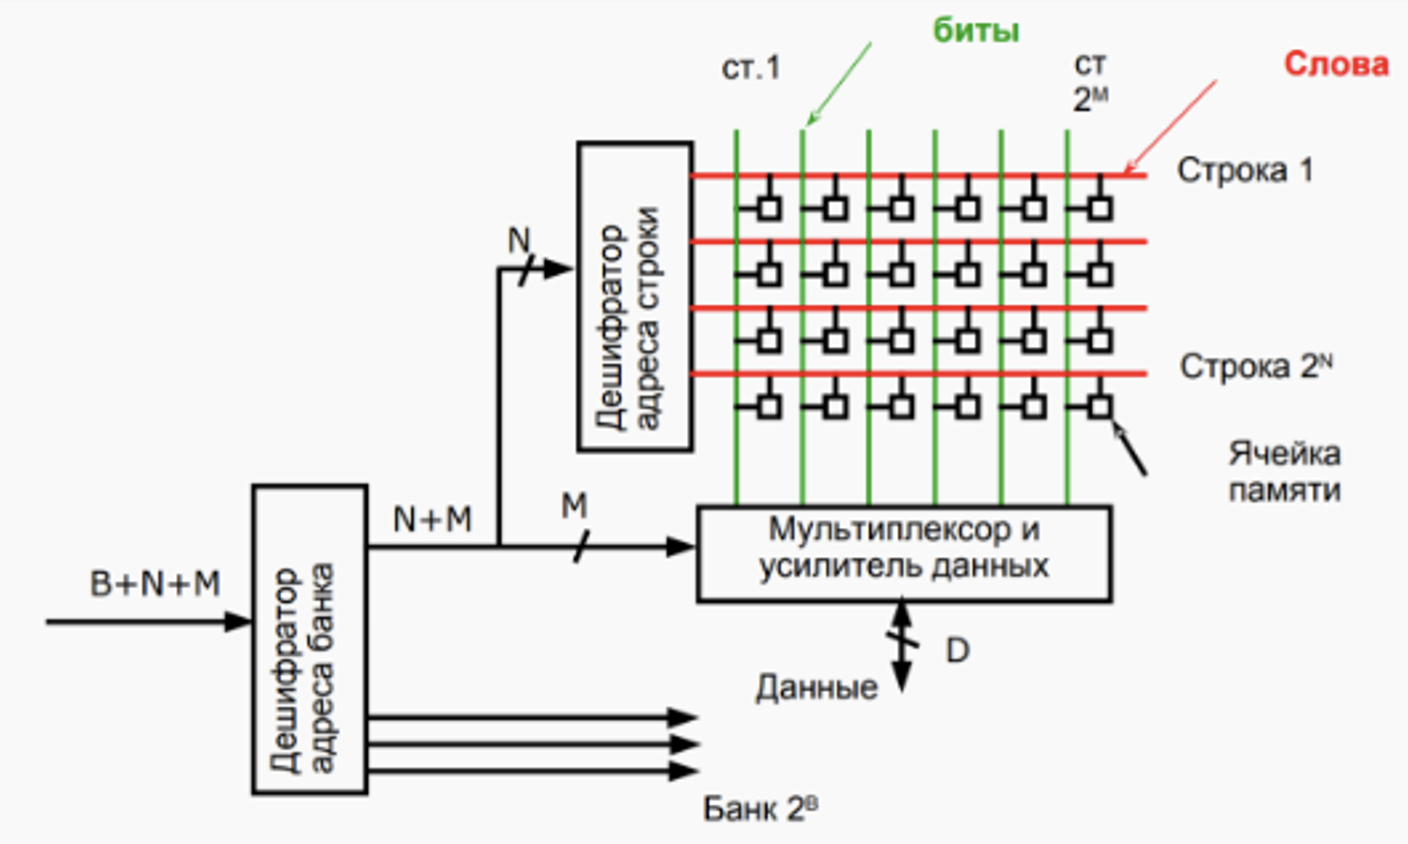
\includegraphics[width=.8\textwidth]{memory_adr.png}\\
Организация адресуемой памяти в реальности отличается от той, которая представлена в бэвм (дешифратор, который обращается к заданной линии). 
В реальности существует мультиплексор – устройство, которое осуществляет передачу сигнала с входа неизменным на выход. 
Входов много, а выходов один. Память разбита на банки, а не является единым пространством. 
Дешифратор выбирает адрес банка, а каждый банк состоит как раз из дешифратора адреса строки и мультиплексора. 
Такая структура существенно проще по сравнению с использованием огромного единого дешифратора.
\\
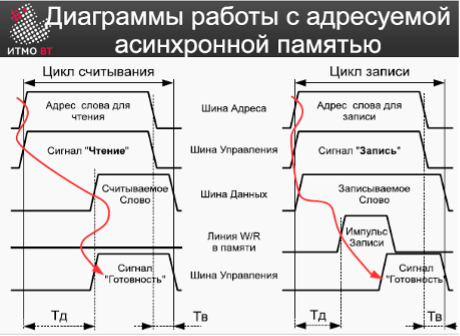
\includegraphics[width=.8\textwidth]{addr_mem.png}\\
Цикл считывания и записи разные, разные управляющие сигналы, которые подаются в разные моменты времени. 

Цикл считывания: при поступлении сигнала для чтения до момента получения данных из памяти пройдет какое-то время, 
за которое произойдет обращение сначала к дешифратору банка, потом адреса и мультиплексора, и только после этого данные будут считаны. 
Одновременно с данными обычно поступает сигнал готовности. 
После этого процессор читает данные и снимает с шин адрес для чтения и сигнал для чтения, 
вследствие чего считываемое слово пропадет с шины данных. Наступает время восстановления.


Цикл записи: выставляется на шину адрес записи, на шину управления сигнал записи, на шину данных выставляется записываемое слово. 
Срабатывают дешифраторы, внутри памяти формируется импульс записи. 
Формируется сигнал готовности, с шин снимаются сигналы и данные, наступает время восстановления.


Было решено разбить адрес на условно адрес строки и адрес столбца и передавать их последовательно по шине. 
Схема с банком не изменилась, добавились 2 доп регистра и 2 сигнала: RAS – выбор строки и CAS – выбор столбца. 

Конструктивные особенности современной памяти:

Burst mode – после первой подачи адреса каждое следующее слово выдается последовательно из памяти;

передача данных по фронту и спаду импульса;

SPD – чип, содержащий идентификационную информацию о памяти;  

несколько димов памяти располагаются не параллельно, а последовательно, засчет чего увеличивается возможное машинное слово;

\section{Память, ориентированная на записи (блочная память). Организация дисковой памяти и памяти на магнитных лентах}
Блочная структура: Адресное пространство памяти разбивается на группы последовательных адресов, и каждая такая группа обеспечивается отдельным банком памяти.

Жесткие диски:  поверхности из блинов, на которой записана информация и головоки, которые читают информацию с намагниченной поверхности, 
когда головка идет по диску (диск разбит на секторы, содержащие преамбулы говорящие о начале сектора, информацию (512 байт/сектор) и поле для контроля четности). 
Время доступа к диску определяется по той самой формуле.

Т позиционирования (двигаем головку) + Т поворота до нужного блока (крутим диск)


Далее берем среднее поскольку каждый раз блок находится на разном расстояние от текущего положения головки.

Ленточные же накопители обладают дешевой стоимостью хранения информации. За счет поворота головки данные записываются на ленту под углом, что увеличивает скорость передачи данных. 
Затруднена работа посекторно, поэтому информацию располагают сначала, последовательно и без промежутков. 

\section{Характеристики запоминающих устройств. Пирамида памяти}
Характеристики:

1. Месторасположение - процессорные, внутренние, внешние

2. Емкость - В метрических и двоичных множителях

3. Единица пересылки - Слово, строка кэша, блок на диске

4. Метод доступа - Произвольный (адресный), ориентированных на записи (прямой), последовательный, ассоциативный

5. Быстродействие и временные соотношения

а. Время доступа 

b. Длительность цикла памяти 

с. Время чтения и время записи

d. Время восстановления 

е. Скорость передачи информации

6. Физический тип и особенности

7. Стоимость
\\ 

Время доступа - время от обращения до передачи информации.
Время восстановления необходимо для приведения памяти в исходное состояние после того, как процессор снял с шин адрес, сигнал ЧТЕНИЕ/ЗАПИСЬ и данные.


Пирамида памяти:

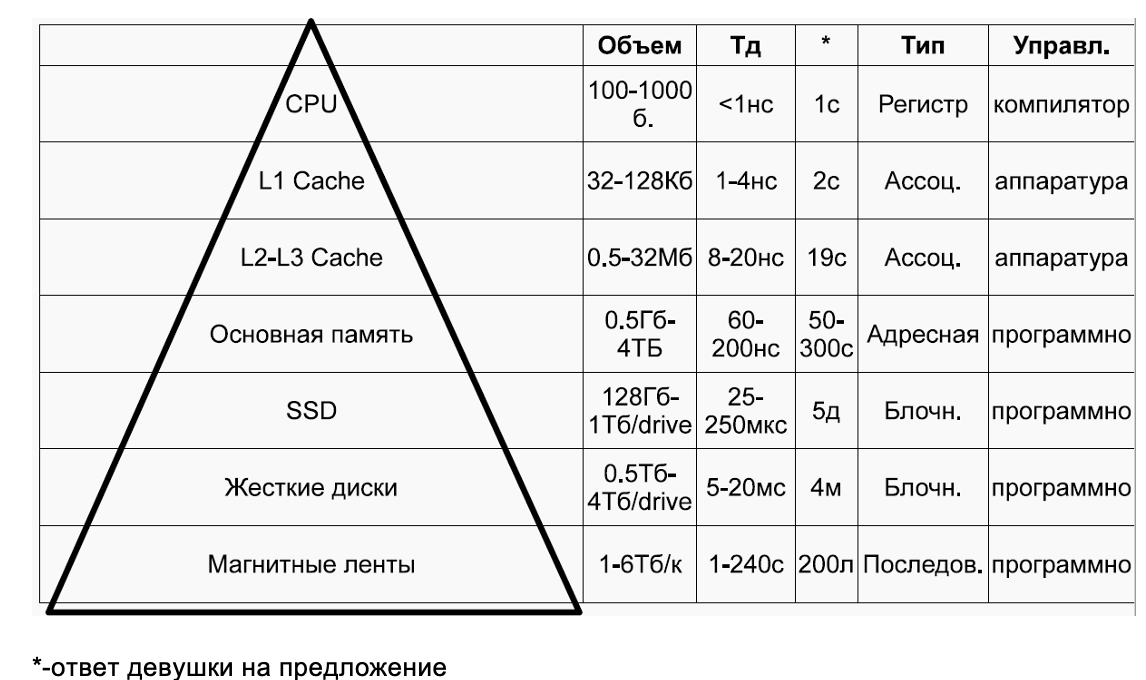
\includegraphics[width=.8\textwidth]{memory.png}

\section{Ассоциативная память, Кэш-память. Влияние промахов кэш-памяти на производительность}
Ассоциативная память построена по следующему принципу, она выбирает не информацию по адресу, а по нужному для нас признаку. 
Т.е у нас есть регистр ассоциативного признака, а каждая ячейка памяти содержит в себе схему сравнения, т.е все что поступает на нее сравнивается 
на наличие необходимого содержимого и те ячейки которые совпадают передаются при помощи регистров сравнения в дальнейшую комбинационную схему.
Компаратор – сравнивающее устройство. Помимо привычных регистров содержит регистры ассоциативного признака, маски, совпадений.
Память такая дорогая за счет компараторов


Кэш-память — это высокоскоростная память произвольного доступа, используемая процессором компьютера для временного хранения информации. 
Она увеличивает производительность, поскольку хранит наиболее часто используемые данные и команды «ближе» к процессору, откуда их можно быстрее получить. Адрес бьется на некоторое количество частей, которые делятся на так называемый тег и просто адрес
В КЭШ памяти выбирается по тег содержимое и потом выдается строка из кэш памяти
Типичная структура записи в кэше: Блок данных, тег, бит актуальности

Кэш-промах – когда приложение запрашивает данные, которых в кэше нет, так что для помещения их в кэш нужно обратиться к диску. 
Чем меньше кэш промахов, тем лучше функционирование системы и производительности. К примеру, при 98\% попадания в кэш производительность
 падает до 60\% по сравнению со 100\% попаданий.


\section{Предназначение и организация виртуальной памяти. Сегментно-страничная организация. Устройство управления памятью (MMU), буфер трансляции (TLB).}

Виртуальная память - технология управления памятью ЭВМ, благодаря которой операционная система может обращаться к памяти, большей, чем память, фактически установленная в компьютере. 
Метод основан на идее, что объединенный размер программы, данных и стека может превышать количество доступной физической памяти, в связи с этим операционная система хранит части программ, 
используемые в настоящий момент, в оперативной памяти, остальные - на диске.
Это достигается за счет помещения данных в свободное дисковое пространство внешнего ЗУ, которое задействовано в роли оперативной памяти. 
Необходимо понимать, что часть программ, которые мы не смогли разместить в оперативной памяти из-за её нехватки, 
теперь будут размещены на ВЗУ и это будет эквивалентно размещению в оперативной памяти. 
Основное назначение - каждая программа думает, что работает в собственном адресном пространстве.


Сегментно-страничная виртуальная память:


Данный метод организации виртуальной памяти направлен на сочетание достоинств страничного и сегментного методов управления памятью. 
В такой комбинированной системе адресное пространство пользователя разбивается на ряд сегментов по усмотрению программиста. 
Каждый сегмент в свою очередь разбивается на страницы фиксированного размера, равные странице физической памяти. 
С точки зрения программиста, логический адрес в этом случае состоит из номера сегмента и смещения в нем. 
С позиции операционной системы смещение в сегменте следует рассматривать как номер страницы определенного сегмента и смещение в ней.

MMU – устройство, на вход поступает виртуальный адрес, есть специальная таблица преобразований, которая говорит есть ли данная страница в виртуальной 
памяти и какой у нее адрес физической памяти. Манипулирование таблицей осуществляет ОС. 

TLB – устройство. Туда записываются виртуальные адреса и соответствующие им физические, т.е кэширует готовый мапинг для часто используемых программ. 
Организован в виде ассоциативной памяти.  


\section{Сетевые технологии, Понятие сети ЭВМ, классификация компьютерных сетей. Сообщение и пакет. Модель взаимодействия открытых систем.}
Сетевая технология – согласованный набор стандартных протоколов и реализующих их программно-аппаратных средств, достаточных для построения сетей эвм.
Понятие сети ЭВМ:

Средства вычислительной техники (СВТ): ЭВМ, вычислительные комплексы (ВК) и вычислительные системы (BC) - реализуют обработку данных.


Средства телекоммуникаций (связи) (СТК): совокупность каналов связи и каналообразующей аппаратуры - реализуют передачу данных.


Сеть ЭВМ (вычислительная сеть, компьютерная сеть) = СВТ+CTK

Классификация компьютерных сетей: данные сети можно разделить по некоторым свойствам

1. По размеру (PAN, LAN, MAN, WAN)

2. По принадлежности (Офисные, корпоративные, чатсные vpn)

3. По назначению (Вычислительные, Информационные, Информационно-вычислительные, Информационно-управляющие)

4. По области применения (SAN - Сети хранения данных, Серверные фермы)

5. Прочие (Иерархические, Беспроводные, Виртуальные VLAN)


Сообщение и пакет:

Длинные сообщения бьются на пакеты (обычно 1500 байт). 
Каждое сообщение и пакеты содержат заголовок (соответствует уровню передач, содержит IP, служебную информацию о портах, адреса отправления и назначения), 
данные и концевик (контрольная сумма по которой производится проверка полученных данных).

Модель взаимодействия открытых систем:
\\
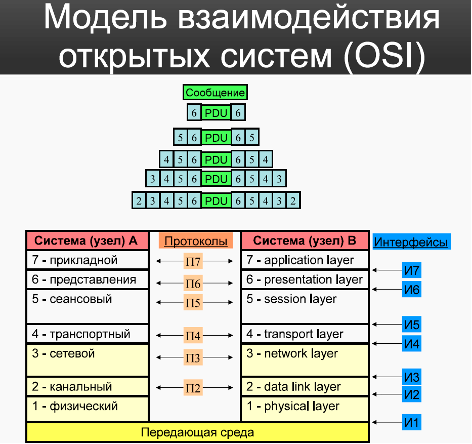
\includegraphics[width=.8\textwidth]{osi.png}\\
Для организации обмена по сети была придумана эталонная 7-уровневая модель взаимодействия систем. 
По мере понижения уровней сообщение обворачивается в дополнительный заголовок. 
На нижних уровнях присутствует заголовок всех предыдущих уровней. 
После передачи в другую систему в обратном порядке эти заголовки разворачиваются. 

\section{Модель TCP/IP: передающая среда, канальный и сетевой уровень. Адресация, передача и маршрутизация пакетов.}

Сетевой уровень (IP) – главная задача передавать пакеты между узлами сети. На сетевом уровне все наши служебные пакеты и пакеты с данными преобразуются в IP gatagramm: 
туда добавляются IP адреса, служебная информация и др. С помощью этого уровня проходит пересылка данных между несколькими маршрутизаторами. 
На сетевом уровне адреса задаются с помощью IP адресов, которые разбиты на 2 части: один определяет номер сети для групповой маршрутизации, 
другой – хоста внутри сети.

Маршрутизация – для установления соединения с заданным адресом нужно сформировать пакет для отсылки по сети. 
Берётся из таблицы маршрутизации запись, соответствующая локальному сегменту сети, далее нужно узнать МAC адрес для его пересылки. 
Если же передача данных осуществляется адресу, не входящему в локальную сеть, передача переключается на роутер по умолчанию в нашей локальной сети. 
Происходит запрос всем локальным адресам, с помощью которого машина получает нужный адрес из роутера. 
Пакет дооформляется IP адресами, уровень MAC добавляется нужными MAC-адресами. Пакет попадает на роутер, который разворачивает его MAC адреса и получает IP. 
По собственной таблице маршрутизации пакет оборачивается другими MAC адресами и отправляется на сервер и распаковывается, обрабатывается и по тому же пути отправляется на нашу локальную машину. 

Канальный уровень – каждый пакет на уровне IP преобразуется в пакет канального уровня на уровне Ehternet. 
Состоит из преамбулы, адресов назначения и источника (MAС адреса, состоят из 6 байт информации, которые прошиты в устройстве и остаются неизменными), 
тип пакета и полезной нагрузки, содержащей протоколы высокого уровня. 
Попадает в передающую среду и передается с одной физической машины на другую. 

Передающая среда:

•	Коаксиальный кабель – антенна, надежность которой оставляла желать лучшего. При разрыве происходило разделение сети на 2 части, которые не видели друг друга.

•	Витая пара – появились свичи, коммутаторы, с помощью которых кабель был подключен к каждому компьютеру. При поломке одного кабеля ломалась не вся сеть, а конкретный узел. 
Преимущество в появлении индукции и распространении сигнала в обе стороны, за счет чего помехи взаимно уничтожаются.  

•	Оптика – при подключении из кабеля светится лазерный луч, излучающее устройство SFP, имеет возможность передачи на дальние расстояния. 

•	Wireless – привычный нам WIFI и мобильный интернет. Беспроводная передача информации. 


\section{Модель TCP/IP: выделение адресов (DHCP), сервисы имен, транспортный и прикладной уровни.}
Прикладной уровень – состоит из приложения на локальной машине и приложения на другой вычислительной машине, к которому мы обращаемся (веб-сервер). 
Общение с удаленной системой имеет аналогию взаимодействия чтения из файла и записи в него. 
С практической точки зрения любой веб-браузер обращается к серверу, устанавливает соединение и выкачивает необходимую нам информацию.


Транспортный уровень (TCP) – сообщение разбивается специальными драйверами на пакеты данных. 
Этот уровень организует виртуальный канал, для которого посылает огромное количество служебных пакетов. 
Сначала запрос на соединение, на которое сервер отвечает разрешением или отказом. 
В случае разрешения посылается на сервер еще одно подтверждение, что разрешение принято и начинается передача данных пакетами.
Для закрытия соединения посылаются соответствующие пакеты, на которые сервер также отвечает, что этот запрос принят и соединение с его стороны прервано. (http, ftp, ssh, smtp)
Кроме TCP протокола существует UDP.(snmp, tftp, dhcp, dns) Разница состоит в том, что TCP медленный и требует установления соединения и его завершения, а UDP этого не требует и на практике просто послал пакет и забыл, быстрый.

DHCP – протокол, позволяющий выдавать IP адреса автоматически. 

Для преобразования IP адресов во что-то более понятное для человека был придуман сервис имен. Концепция DNS построена иерархическим путем: есть корневые серверы в сети интернет, которые содержат зоны, каждая из которых содержит свои name сервера, которые содержат информацию локально.
При этом сервис имен не ограничивается DNS. Кроме имен машин нужно еще хранить имена пользователей, групп, номера телефонов. К таким серверам относится LDAP, предназначенный для хранения всего. 

\section{Интерфейсы ввода-вывода. Контроллеры внешних устройств. Уровни стандартизации, сопряжения с системной шиной, циклы обмена. Регистры контроллера.}
Интерфейсы определяют частоту, набор каналов передачи, способ кодирования, команды, представление данных, набор данных и последовательность.
Требуется аппаратная и программная реализация.

Уровни стандартизации: Логическое подключение; Физические параметры сигналов; Конструктивные особенности

Сопряжение с системной шиной происходит через контроллер ВУ. Сопряжение устройств с ЭВМ состоит из двух уровней сопряжения: Процессор (работает отдельно) и какой-либо набор сигналов, который формирует системную шину, которая сопрягает их системно с контроллерами; второй уровень сопряжения между контроллером и ВУ при помощи переферийных шин.
2 режима обмена информацией с контроллерами ВУ: Программно-управляемый, Прямой доступ в память. 


При использовании для обмена с ВУ команд ввода-вывода, адрес ВУ передается по шине адреса. 
По этой же шине передаются и адреса ячеек памяти.
При реализации обмена с ВУ по аналогии с обращениями к памяти нет необходимости в спец. сигналах. 
В контроллерах организована селекция адресов ВУ. 
Остается передавать приказ на ввод/вывод информации. 
Для этого есть линии управляющей шины «Чтение» и «Запись».


Операция вывод: микропроцессор выставляет на линиях адресной шины адрес ВУ, на линиях шины данных - значения разрядов выводимого слова данных и единичный сигнал «Вывод». 
Адресуемый контроллер ВУ принимает данные, пересылает их в ВУ и сигналом «Ґотовность ВУ»
сообщает процессору, что данные приняты и можно снять информацию с шин адреса и данных, а также сигнал «Вывод».


Операция ввод: микропроцессор выставляет на линиях адресной шины адрес ВУ, и единичным сигналом на линии «Ввод» указывает тип операции. 
По сигналу «Ввод» контроллер считывает слово данных из ВУ, выставляет на линиях шины данных значения разрядов считанного слова и единичным сигналом на линии
«Готовность ВУ» сообщает об этом процессору. Приняв данные, процессор снимает сигналы с шины адреса и линии «Ввод».


Рассмотрим типичные структуры контроллеров ВУ:

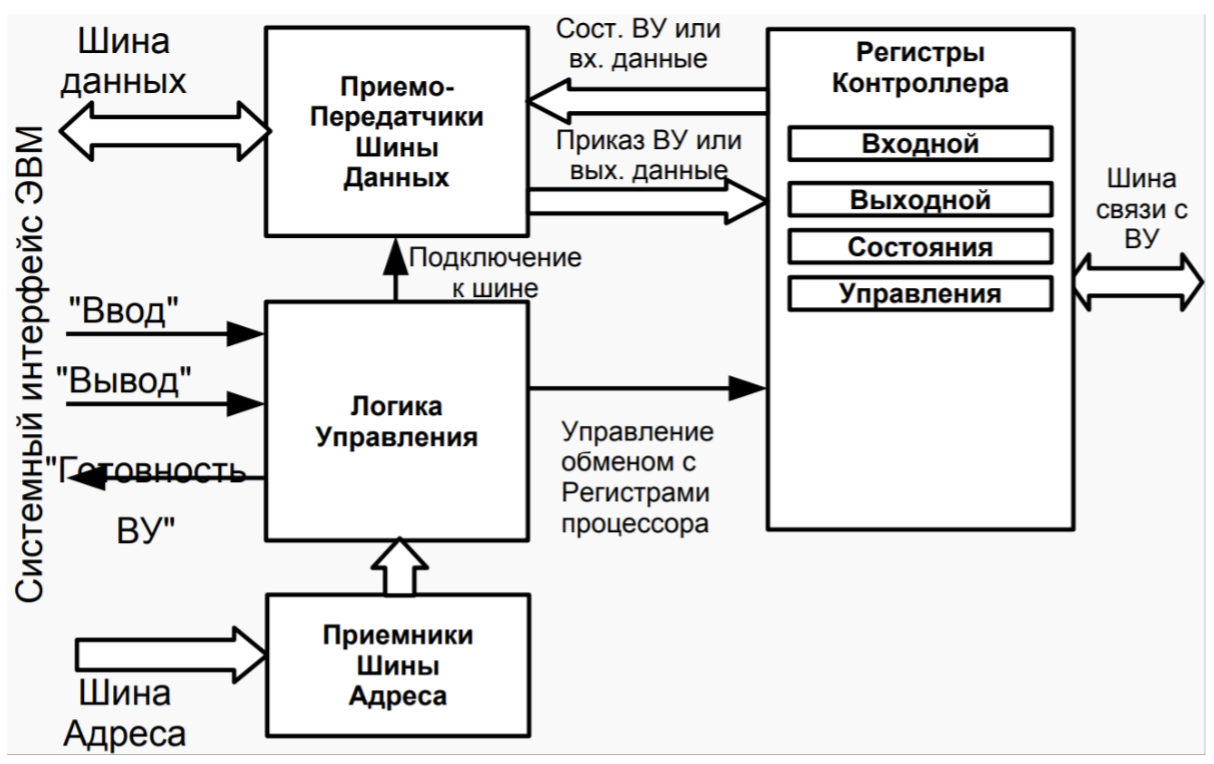
\includegraphics[width=.8\textwidth]{kontr-bu.png}

\textbf{Описание схемы:}

Слева сверху располагаются приемопередатчики шины данных, ниже логика управления, ниже приёмники шины адреса. Правее располагаются регистры контроллера, в этом блоке есть входной, выходной, состояния, управления. 
Двунаправленная шина данных идёт от интерфейса эвм к приемопередатчикам. От логики управления к приемопередатчики идёт провод. От интерфейса эвм к логике приходят провода: ввод и вывод и исходит провод готовности ву. 
Шина адреса подходит к приёмникам шины адреса. От них выходит шина до логики управления.

К регистрам контроллера подходит двунаправленная шина от ву. От логики управления выходит провод (Управление обменом с регистрами процессора) до регистров контроллера. От регистров контроллера выходит шина к приёмо передатчикам(Состояние ву или вх данные). От приёмопередатчиков выходит шина до регистров контроллера.
\section{Параллельная передача данных. Контроллеры параллельной передачи и приема.}
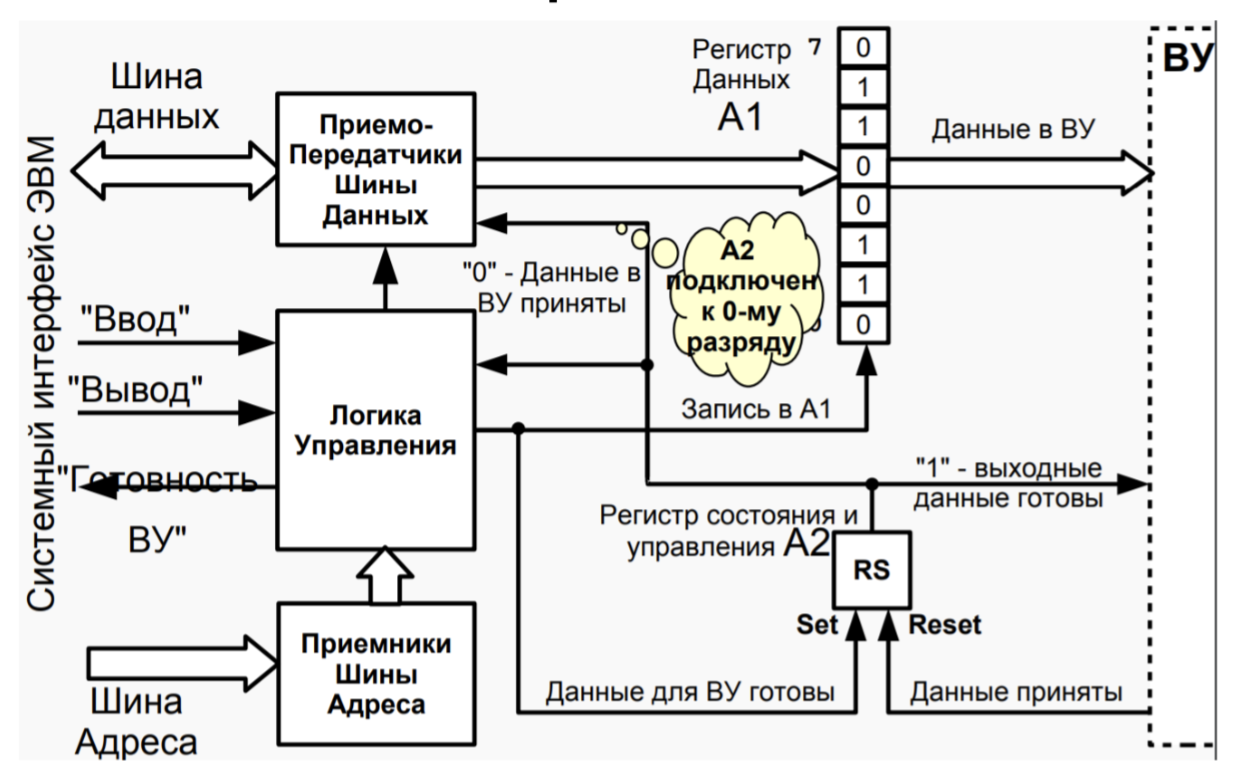
\includegraphics[width=.8\textwidth]{out1.png}\\
\textbf{Описание контроллера:}
Слева сверху располагаются приемопередатчики шины данных, ниже логика управления, ниже приёмники шины адреса. Двунаправленная шина данных идёт от интерфейса эвм к приемопередатчикам. От логики управления к приемопередатчикам идёт провод. От интерфейса эвм к логике приходят провода: ввод и вывод и исходит провод готовности ву. 
Шина адреса подходит к приёмникам шины адреса. От них выходит шина до логики управления. 
Правее располагается регистр данных А1 вертикально с 8 разрядами, от 0 до 7 вверх. Ниже раположен рс триггер - регистр состояния и управления А2. 
От логкик управления идёт провод к регистру данных А1 в 0 бит и этот же провод идёт на вход set триггера. От ву идёт провод информирующий что данные приняты на рс триггер. От рс триггера исходит провод, который идёт на ву (если 1, то данные готовы) и (если ноль, то данные приняты) на приёмопередатчики и на логику управления.
А2 подключен к нулевому разряду А1



Параллелность и заключается в том, что данные передаются по 8 разрядной шине данных, то есть сразу всё, по одному сигналу готовности.\\

Сам алгоритм: \\
Параллельная передача данных в ВУ под управлением программы асинхронного обмена:

1. Процессор проверяет готовность ВУ к приему данных

2. Если ВУ готово к приему данных, то данные передаются из шины данных системного интерфейса в регистр данных А1 контроллера и далее в
ВУ. Иначе повторяется пункт 1.

В шине связи с ВУ используются 2 управляющих сигнала. Для формирования управляющего сигнала «Выходные данные готовы» и приема из ВУ управ сигнала «Данные приняты» в контроллере используется одноразрядный адресуемый регистр состояния и управления А2. 
Одновременно с записью очередного байта данных в адресуемый регистр данных контроллера А1 в регистр состояния и управления записывается логическая единица (формируется управляющий сигнал«Выходные данные готовы»).
ВУ, приняв байт данных, управ. сигналом «Данные приняты» обнуляет регистр состояния.
В логике управления - селекция адресов регистров контроллера, прием и формирование управ. сигналов, формирование сигнала «Готовность ВУ».
Для сопряжения регистров контроллера с шинами адреса и данных сист. интерфейса используются приемники шины адреса и приемопередатчики шины данных.\\

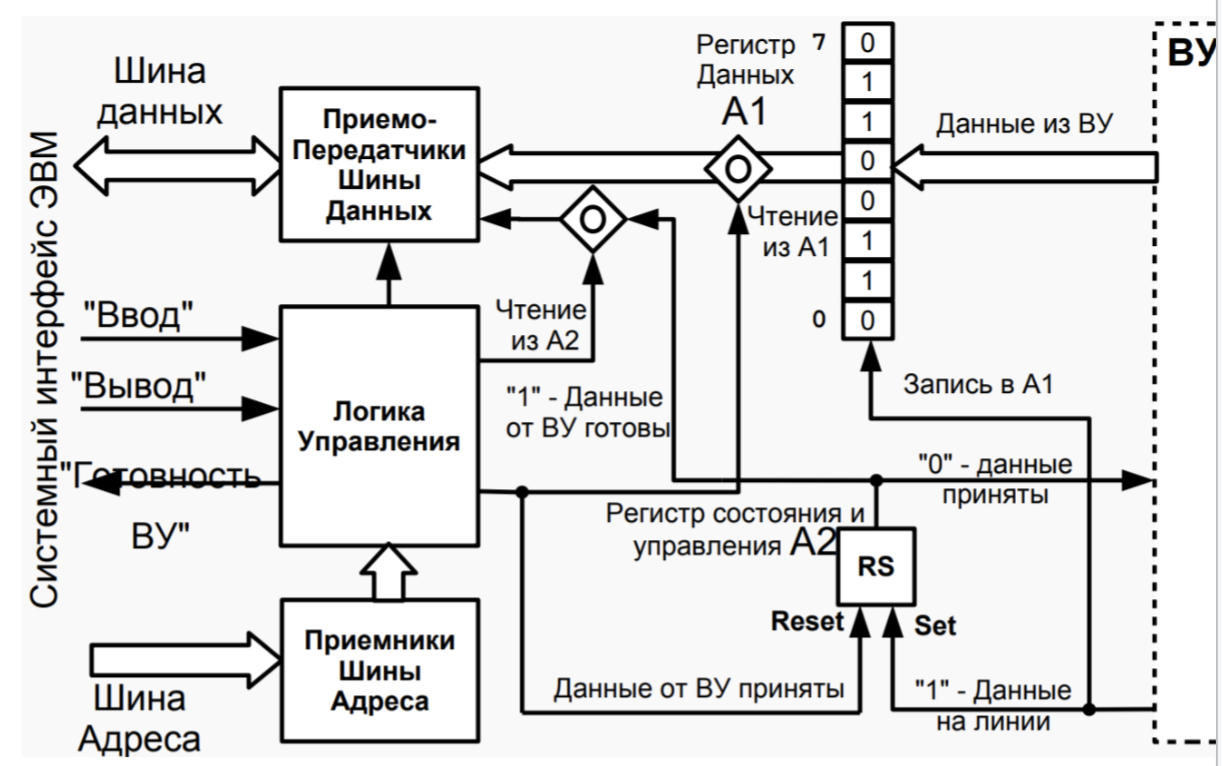
\includegraphics[width=.8\textwidth]{in1.png}\\
\textbf{Описание контроллера:}
Слева сверху располагаются приемопередатчики шины данных, ниже логика управления, ниже приёмники шины адреса. Двунаправленная шина данных идёт от интерфейса эвм к приемопередатчикам. От логики управления к приемопередатчикам идёт провод. От интерфейса эвм к логике приходят провода: ввод и вывод и исходит провод готовности ву. 
Шина адреса подходит к приёмникам шины адреса. От них выходит шина до логики управления. 
Правее располагается регистр данных А1 вертикально с 8 разрядами, от 0 до 7 вверх. Ниже раположен рс триггер - регистр состояния и управления А2. 
От ву идёт шина данных к А1, от А1 идёт шина к приемопередатчикам через вентиль. 
Из логики управления идёт провод до этого вентиля (чтение из А1), этот провод также идёт на вход reset триггера (данные от ву приняты).
От ву идёт провод в нулевой бит А1 (запись в А1) и этот же провод идёт на вход сет триггера (данные на линии).
От рс триггера идёт провод на ву (0 данные приняты) и через новый вентиль на приемопередатчики. К этому вентилю подходит провод от логики управления(чтение из А2)
\\ \\
Алгоритм асинхронного ввода:

1. Процессор проверяет наличие данных в регистре данных контроллера А1

2. Если данные готовы, то они передаются из регистра данных А1 в шину данных системного интерфейса и далее в регистр процессора или ячейку памяти микроЭВМ. 

Иначе повторяется пункт 1.

Для формирования управляющего сигнала «Данные приняты» и приема из ВУ управ. сигнала «Данные от ВУ готовы» в контроллере используется одноразрядный адресуемый регистр состояния и управления А2.
ВУ записывает в регистр данных контроллера А1 очередной байт данных и управ. сигналом

«Данные от ВУ готовы» устанавливает в единицу регистр состояния и управления А2. При этом формируется:

1. Управ. сигнал сист. интерфейса «Готовность ВУ»

2. Признак готовности ВУ к обмену, передаваемый в процессор по одной из линий шины
данных

Так контроллер извещает процессор о готовности данных в регистре А1. Процессор читает байт данных из регистра данных контроллера и обнуляет регистр состояния и управления
A2. При этом формируется управляющий сигнал «Данные приняты».

\section{Синхронные последовательные интерфейсы. Контроллеры последовательной передачи и приема.}
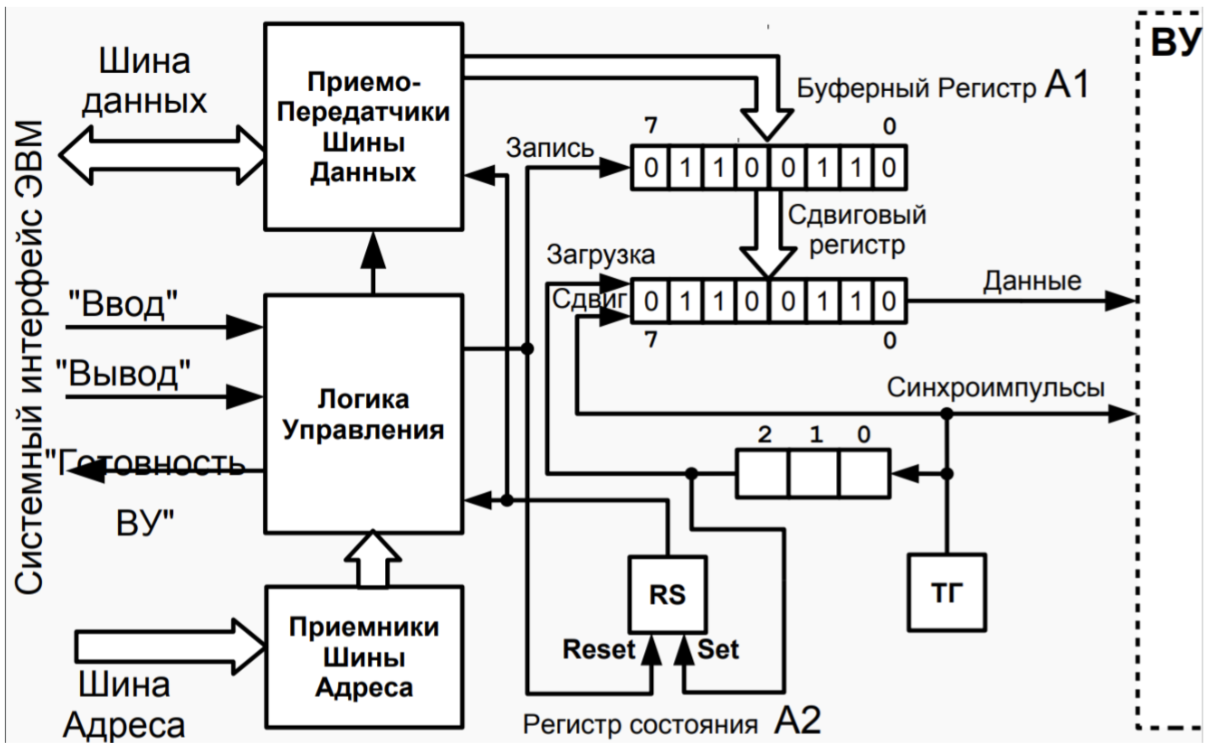
\includegraphics[width=.8\textwidth]{out2.png}\\
\textbf{Описание контроллера:}
Слева сверху располагаются приемопередатчики шины данных, ниже логика управления, ниже приёмники шины адреса. Двунаправленная шина данных идёт от интерфейса эвм к приемопередатчикам. От логики управления к приемопередатчикам идёт провод. От интерфейса эвм к логике приходят провода: ввод и вывод и исходит провод готовности ву. 
Шина адреса подходит к приёмникам шины адреса. От них выходит шина до логики управления. 
Правее находится буферный регистр А1 горизонтальный от 7 до 0. Ниже находится сдвиговый регистр горизонтальный от 7 до 0. 
Ниже находится счётчик из 3х ячеек 2, 1, 0.
Ниже нахдятся регистр состояния А2 аля рс триггер и тактовый генератор. 
От логики исходит провод к А1 (Запись) и на вход резет триггера.
От тактового генератора одёт провод до ву(синхроимпульсы), до сдвигового регистра (сдвиг) и до счётчика.
От счётчика идёт провод к сдвиговому регистру(загрузка) и на вход сет триггера.
От триггера исходит провод да логики и до приемопередатчиков.
От приемопередатчиков исхоит шина до А1. 
От А1 идёт шина да сдвигового регистра. 
От него идёт провод (данные) до ву.
\\ \\

Логика работы:

8-ми разрядный буферный регистр контроллера А1 - для временного хранения байта данных до его загрузки в сдвиговый регистр. Запись байта данных в буферный регистр происходит при наличии 1 в регистре состояния А2. Содержимое этого регистра передается в процессор по одной из линий шины данных и используется для формирования управ. сигнала «Готовность ВУ». При записи очередного байта в регистр А1 обнуляется регистр A2.
В сдвиговом регистре происходит преобразование данных из параллельного формата в последовательный и передача их в линию связи. По очередному тактовому импульсу содержимое сдвигового регистра сдвигается на 1 разряд вправо и в линию связи «Данные» выдается значение очередного разряда. Одновременно со сдвигом по линии
«Синхронизация» передается тактовый импульс.
Количество переданных в линию тактовых сигналов (переданных бит) подсчитывается счетчиком тактовых импульсов. Как только его содержимое равно 7(передано 8 бит информации) формируется управляющий сигнал «Загрузка» и происходит запись в сдвиговый регистр очередного байта из буфера. Устанавливается в 1 регистр состояния.
Следующим тактовым импульсом счетчик будет сброшен в 0 и начнется очередной цикл выдачи 8 бит из сдвигового регистра в линию связи.
\\
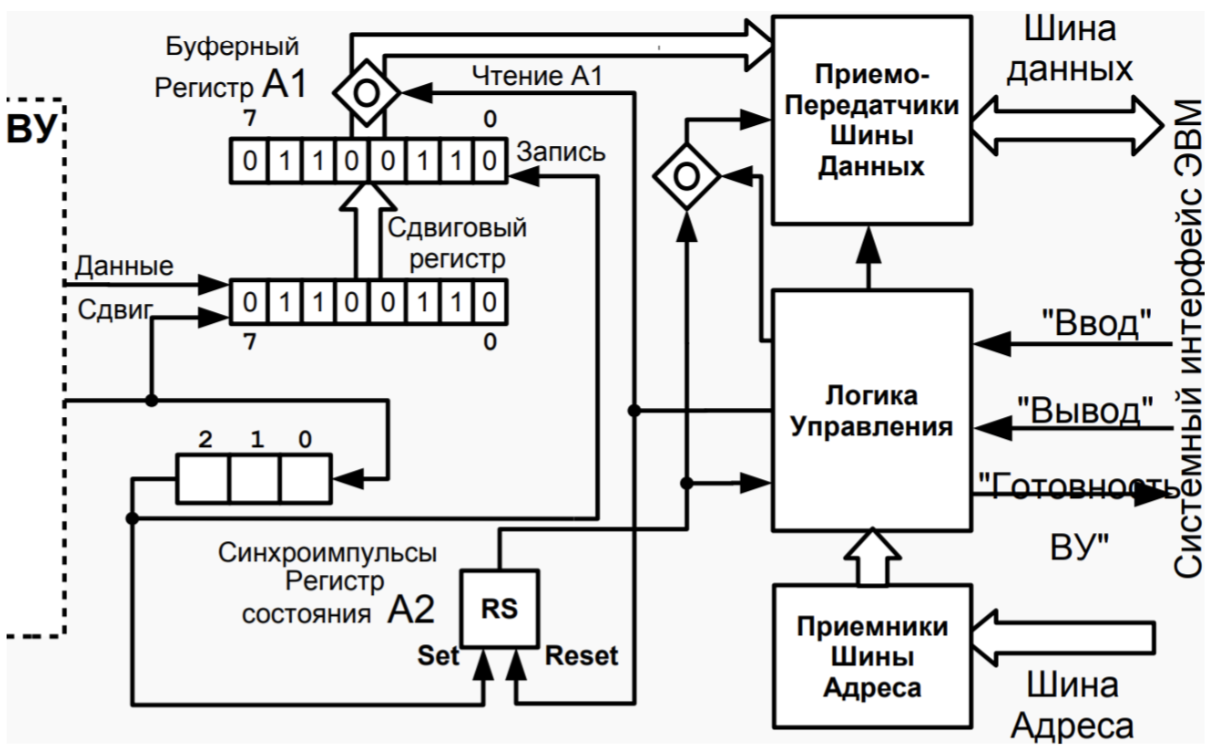
\includegraphics[width=.8\textwidth]{in2.png}\\
\textbf{Описание контроллера:}
Справа сверху располагаются приемопередатчики шины данных, ниже логика управления, ниже приёмники шины адреса. Двунаправленная шина данных идёт от интерфейса эвм к приемопередатчикам. От логики управления к приемопередатчикам идёт провод. От интерфейса эвм к логике приходят провода: ввод и вывод и исходит провод готовности ву. 
Шина адреса подходит к приёмникам шины адреса. От них выходит шина до логики управления. 
Левее раположился буферный регистр горизонтальный А1 от 7 до 0, под ним сдвиговый регистр горизонтальный от 7 до 0, ниже счётчик с 3 ячейками 2, 1, 0 и ещё ниже триггер.
От триггера идёт провод до логики управления и к приемопередатчикам через вентиль, к которому ещё приходит провод от логики управления.
От сдвигового регистра идёт шина к буферному и от буферного идёт шина через новый вентиль до приемопередатчиков.
От логики управления идёт провод до этого вентиля(чтение А1) и до входа резет на триггере.
От ву идёт провод (данные) к сдвиговому регистру и ещё один провод от ву идёт на самую правую ячейку счётчику, а так же по пути он соединяется к сдвиговому регистру(сдвиг).
От счётчика идёт провод да А1 на правый бит(запись) и на вход сет триггера 
\\
Алгоритм работы:

Буферный регистр контроллера А1 - для временного хранения байта , поступившего из сдвигового регистра. Чтение байта данных из буферного регистра происходит при наличии 1 в регистре состояния А2.
Данные, поступающие из линии связи в последовательном коде преобразуются в параллельный с помощью сдвигового регистра. Линия «Данные» подключается в контроллере к последовательному входу сдвигового регистра, а линия «Синхронизация» - на управ. вход «Сдвиг» и на вход счетчика тактовых импульсов. По тактовому импульсу по линии «Синхронизация» производится сдвиг содержимого сдвигового регистра на 1 разряд вправо и запись очередного бита данных из линии «Данные» в младший разряд этого регистра. Одновременно увеличивается на 1 счетчик тактовых импульсов. Как только он становится равным 7 формируется управ. сигнал «Запись» и происходит запись в буферный регистр байта из сдвигового. Устанавливается в 1 регистр состояния.
При передаче байта данных из буферного регистра в шину данных регистр состояния обнуляется (т.е. в сдвиговый регистр принимается очередной байт информации).

\section{Асинхронный обмен. Принципы деления частоты, формат кадра.}

При реализации асинхронного обмена интервал между командами передачи данных задается самим внешним устройством. 
Контроллеры этих устройств снабжаются регистром состояния, который информирует ЭВМ о готовности устройства к обмену информацией.
Обмен происходит по готовности ВУ.

Преимущества:

1. Не нужно знать время выполнения операции на ВУ;

2. ВУ всегда успеет выполнить обработку данных перед началом следующей операции обмена.

Недостаток - ЭВМ не выполняет никаких полезных действий во время ожидания момента готовности ВУ.

При асинхронной передаче данных, со временем может происходить рассинхронизация генераторов тактов передатчика и приёмника, в результате чего данные могут быть переданы с искажениями, или не быть переданы вовсе.
Одним из способов решения этой проблемы является деление тактовой частоты генераторов.
Принцип его заключается в том, что исходная тактовая частота делится с некоторым коэффициентом, чаще всего делят не меньше, чем на 16. 
Таким образом увеличивается область совпадения фаз и время передачи данных, что увеличивает точность передачи.
Очень часто необходимо использовать триггер для деления частоты входной последовательности импульсов на два, т. е. производить переключение триггера в новое состояние каждым входным импульсом (фронтом или спадом). 
Такой триггер называют счетным, или T-триггером.
Формат кадра – количество бит стартовых бит, количество бит информации, количество стоповых бит. В кадре может содержаться дополнительная информация, такая, как длина кадра и тд.
\section{Контроллер передачи асинхронного последовательного интерфейса.}
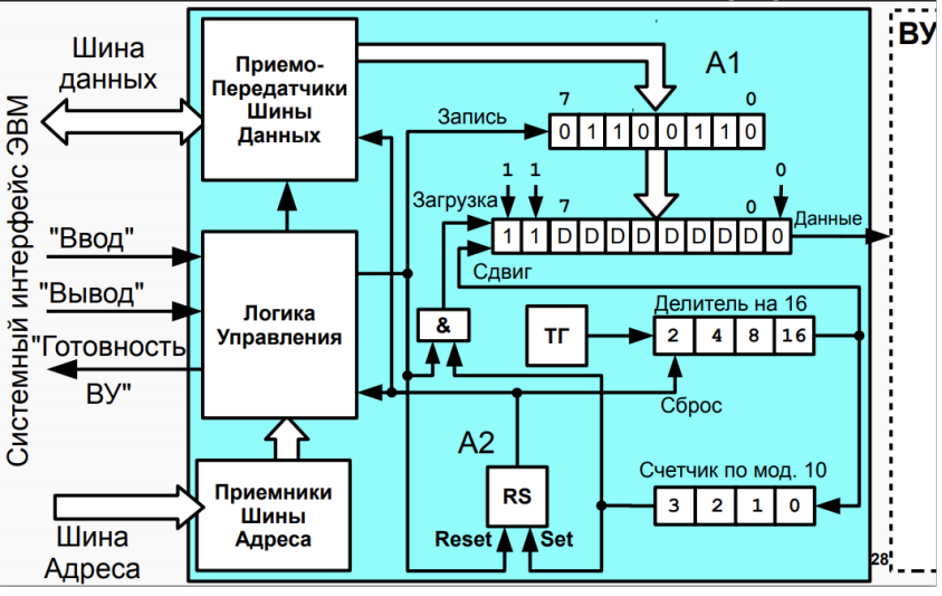
\includegraphics[width=.8\textwidth]{out3.png}\\
\textbf{Описание контроллера:}
Начнём с блока приёмо передатчиков шины данных, ниже него располагается логика управления ещё ниже располагается приёмники шины адреса. Справа есть буферный регистр на 7 значений, горизонтальный. Ниже него есть сдвиговый регистр, где в начале стоит две единицы, далее 8 свободных ячеек и в конце 0. Ниже сдвигового регистра сначала идёт блок с лагическим и, правее тактовый генератор и ещё правее делитель на 16 с ячейками 2,4,8,16. Ниже расположен рс тригер А2 и правее счётчик по модулю 10 с ячейками 3,2,1,0.
Первая шина идёт от эвм к приёмо передатчикам. К логике управления идёт 2 провода провода, ввод и вывод. От логики управления идёт провод готовности ву к эвм, а так же провод к приёмо передатчикам. К приёмникам шины адреса идёт шина адреса и от них идёт шина к логике управления.
От приёмо передатчиков идёт шина к буферному регистру от буферного регистра к сдвиговому. 
От тактового генератора идёт провод к делителю на 16, от делителя на 16 идёт провод к сдвиговому регистру под названием сдвиг и ещё один провод к счътчкиу по модулю 10. От сдвигового регистра идёт один провод к ВУ с данными. К этому регистру в местах 11 и 0 подходят соответсвующие значения.
От счётчика по модулю 10 идёт провод на вход триггера сет и на блок логического и. От логики управления идёт провод к буферному регистру на запись, к блоку логического и, и на вход резет триггера. От логического и идёт провод к сдвиговому регистру. От тригера идёт провод в логику управления, в приёмо передатчик и к делителю на 16 сброс.

\textbf{Логика работы}\\
-	После передачи предыдущих байтов данных в Регистр Состояния А2 записывается 1, что информирует процессор о готовности контроллера к приему следующего байта данных и передаче его по линии связи в ВУ. Он же запрещает формирование импульсов со схемы выработки импульсов сдвига – делителя частоты тактового генератора на 16 (счетчик по mod 16). Счетчик импульсов сдвига (счетчик по mod 10) находится в нулевом состоянии, и его единичный выходной сигнал поступает на вентиль И, подготавливая цепь выработки сигнала загрузки сдвигового регистра. 

-	Процессор, выполняя команду «Вывод», выставляет передаваемый байт на шине данных и формирует управляющий сигнал системного интерфейса «Вывод».

-	По сигналу «Вывод» в контроллере происходит запись передаваемого байта в буферный регистр А1, сброс регистра состояния А2 и формирование на вентиле И сигнала «Загрузка».

-	Передаваемый бит переписывается в разряды 1..8 сдвигового регистра, в 0 разряд записывается нуль – стартовый бит, а в разряды 9 и 10 единицы – стоповые биты

-	Снимается сигнал «Сброс» с делителя частоты, он начинает накапливать импульсы генератора тактовой частоты и в момент приема шестнадцатого тактового импульса срабатывает импульс сдвига (так реализовано деление частоты)

-	На шине «Данные» поддерживается 0 (значение стартового бита) до тех пор, пока не будет выработан первый импульс сдвига (время передачи 1 бита). Импульс сдвига изменит состояние счетчика импульсов сдвига и перепишет в нулевой разряд сдвигового регистра первый информационный бит передаваемого байта данных. Значение этого бита будет поддерживаться на линии «Данные» до следующего импульса сдвига.

-	Аналогично передаются остальные информационные биты, первый стоповый бит, и, наконец второй стоповый бит, при передаче которого счетчик импульсов сдвига снова установится в нулевое состояние. Это приведет к записи 1 в регистр состояния А2. Единичный сигнал с выхода регистра А2 запретит формирование импульсов сдвига, и информирует о готовности к приему нового байта данных.

-	После завершения передачи очередного кадра (стартового бита, информационного бита и двух стоповых битов), на линии передачи данных поддерживается значение второго стопового бита – единицы



\section{Контроллер приема асинхронного последовательные интерфейса}
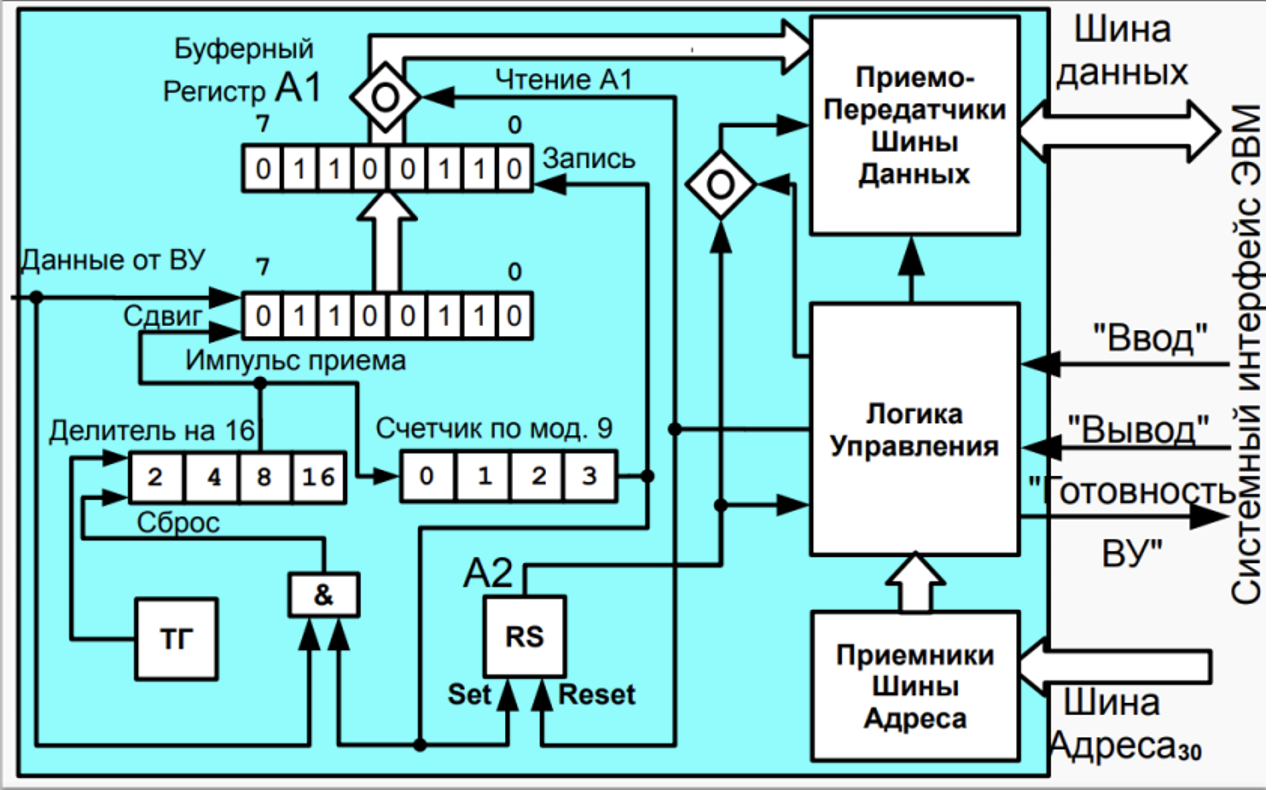
\includegraphics[width=.8\textwidth]{in3.png}\\
\textbf{Описание контроллера:}
Справа сверху располагаются приемопередатчики шины данных, ниже логика управления, ниже приёмники шины адреса. Двунаправленная шина данных идёт от интерфейса эвм к приемопередатчикам. От логики управления к приемопередатчикам идёт провод. От интерфейса эвм к логике приходят провода: ввод и вывод и исходит провод готовности ву. 
Шина адреса подходит к приёмникам шины адреса. От них выходит шина до логики управления.
Левее сверху буферный регистр А1 горизонтальный от 7 до 0, ниже сдвиговый регистр горизонтальный от 7 до 0. Ниже сначала делитель на 16 с ячейками 2, 4, 8, 16 и рядом счётчик по модулю 9 с ячейками 0, 1, 2, 3. 
ниже сначала тактовый генератор, далее блок логичекого и, далее рс триггер А2.
От триггера выходит провод до логики управления  и до приемопередатчиков через вентиль, к которому подоходит провод от логики управления.
От сдвигового регистра идёт шина до А1.
От А1 через новый вентиль идёт шина до приемопередатчиков.
От логики идёт провод на этот вентиль(чтение А1) и на вход резет триггеру.
От тактового генератора идёт провод на левый бит делителя на 16.
От делителя на 16 идёт провод до сдвигового регистра (сдвиг) и до счётчика по модулю 9.
От блока логического и идёт провод до делителя на 16.
От счётчика по модулю 9 идёт провод на А1(запись), а также вниз на вход сет триггера и на блок логичекого и.
От ву идёт провод на сдвиговый регистр (данные от ву) и на логический блок и.

\textbf{Логика работы}\\
1. На линии «Данные» находится единица, что запрещает работу делителя частоты генератора тактовых импульсов.

2. При обнаружении нулевого сигнала на линии «Данные» (смена стопового бита на стартовый), снимается сигнал «Сброс» с делителя частоты, он начинает накапливать импульсы генератора тактовой частоты.

3. Когда на счетчике накопится значение 8 (половина времени передачи бита), он выдаст сигнал, поступающий на входы сдвигового регистра и счетчика импульсов сдвига. (Таким образом уменьшается вероятность искажения данных.)

4. Последующие сдвиги происходят после прохождения 16-ти тактовых импульсов.

5. При приеме в сдвиговый регистр 9-го бита кадра (8-го инф. Бита), из него выдвинется стартовый бит, и, следовательно в сдвиговом регистра будет размещен информационный байт. В этот момент счетчик импульсов сдвига придет в нулевое состояние и на его выходе будет выработан единичный сигнал, по которому:

а. Содержимое сдвигового регистра будет переписано в БР

b. B PC A2 запишется 1 и он будет информировать процессор об окончании приема очередного байта

с. Вентиль И подготовится к выработке сигнала «Сброс»(он сформируется после
прихода первого стопового бита).

6. Получив сигнал готовности (1 в РС A2), процессор выполнит команду «Ввод». При этом
вырабатывается сигнал системного интерфейса «Ввод», по которому производится пересылка принятого байта данных из БР в процессор (сигнал «Чтение») и сброс РС А2




\section{Организация прямого доступа к памяти. Контроллер ПДП.}
Этот тип обмена реализуется полностью аппаратно и управляется контроллером ПДП.
Для экономии ресурсов контроллер ПДП не имеет свои ресурсы, а подключается к шинам данных и адреса системного интерфейса ЭВМ, что делает невозможным одновременное использование шин контроллером ПДП и процессором.
Эта проблема решается двумя способами:
\\ \\
1. Захват цикла

а. Передача происходит в те машинные циклы, в которых процессор не обменивается данными с памятью. 
Пометка таких циклов выполняется либо с помощью спец. указывающего цикла, либо такие циклы выбираются с помощью спец. селектирующих схем, что усложняет конструкцию процессоров. 
Обмен возможен только в случайные моменты времени одиночными байтами или словами.


b. Захват цикла с принудительным отключением процессора от шин системного интерфейса. Системный интерфейс дополняется двумя линиями для передачи управляющих сигналов
«Требование ПДП» и «Предоставление ПДП» .

1. ТПДП формируется контроллером ПДП.

2. Получив сигнал ТПДП, процессор приостанавливает выполнение очередной команды, выдает в системный интерфейс ППДП и отключается от шин СИ

3. Контроллер ПДП получает управления над шинами СИ и осуществляет обмен
одним байтом или словом данных с памятью микроЭВМ.

4. Контроллер ПДП возвращает управление СИ процессору.\\ \\
2. Блокировка процессора. Управление СИ передается контроллеру
ПДП не на время обмена одним байтом, а на время обмена блоком данных.
 \\ \\
 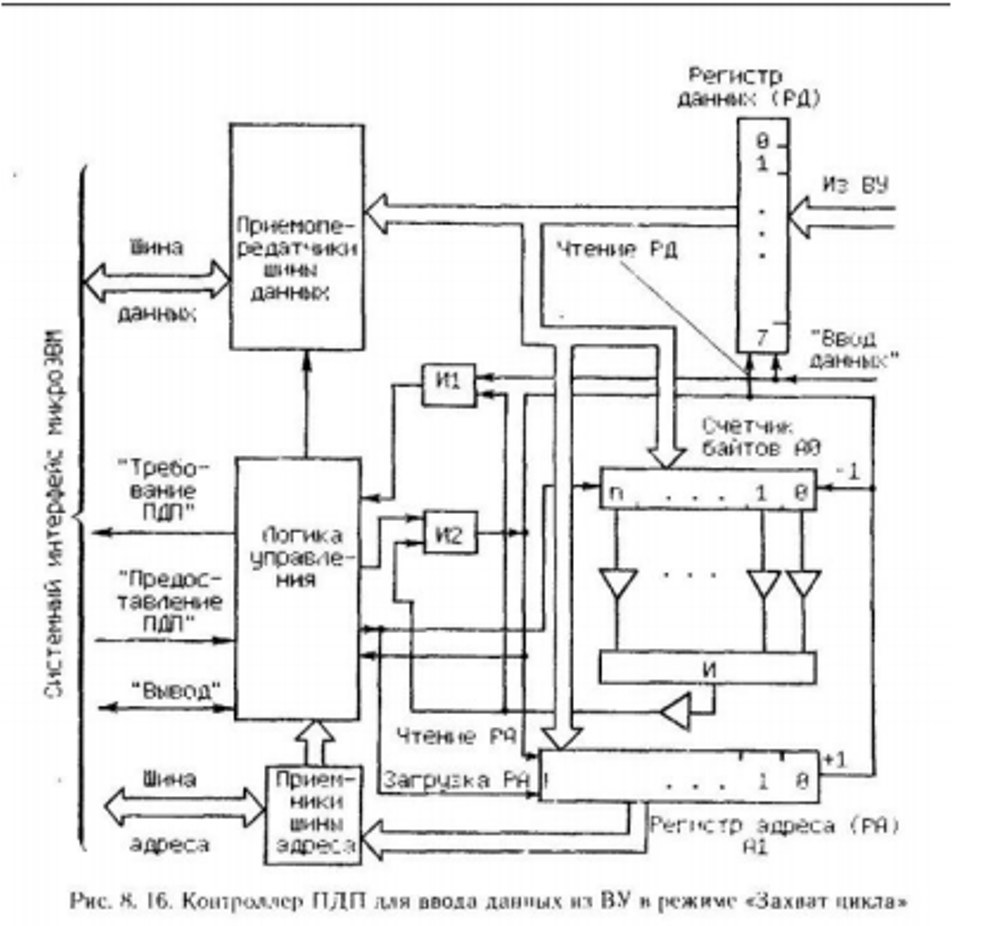
\includegraphics[width=.8\textwidth]{pdp.png}\\
Контроллер ПДП ввода данных из ВУ в режиме «Захват цикла»:

1. Процессор загружает в СК контроллера количество принимаемых байтов, а в РА контроллера начальный адрес области памяти для вводимых данных.

2. Байты данных из ВУ поступают в РД контроллера, при этом каждый байт сопровождается управляющим сигналом из ВУ «Ввод данных», который обеспечивает запись байта в РД контроллера. По этому же сигналу при ненулевом состоянии СК контроллер формирует сигнал ТПДП.

з. По ответному сигналу процессора ППДП контроллер выставляет на ША и ШД содержимое своих РА и РД.

4. Формируя приказ «Вывод», контроллер ПДП обеспечивает запись байта данных из своего регистра данных в память микроЭВМ.

5. По тому же сигналу ППДП содержимое СК декрементируется, а содержимое РА обновляется. Как только СК станет равным нулю, контроллер прекратит формирование сигналов ТПДП
\end{document}
